\documentclass[11pt,a4paper]{report}

%----------------------------------------
% ENCODAGE ET LANGUE
%----------------------------------------
\usepackage[utf8]{inputenc}
\usepackage[T1]{fontenc}
\usepackage[french]{babel}
\usepackage[colorlinks=true, linkcolor=blue, urlcolor=blue, citecolor=blue]{hyperref}

%----------------------------------------
% MARGES : 3 cm
%----------------------------------------
\usepackage[a4paper,
            top=3cm,
            bottom=3cm,
            left=3cm,
            right=3cm]{geometry}

%----------------------------------------
% POLICE : Times (ou proche) + taille de base 11 pt
%----------------------------------------
% Option 1 : newtxtext (recommandé pour Times-like)
\usepackage{newtxtext,newtxmath}

%----------------------------------------
% AUTRES PACKAGES UTILES
%----------------------------------------
\usepackage{footnote}    % pour la gestion des notes de bas de page
\usepackage{graphicx}    % pour \includegraphics
\usepackage{wrapfig}     % pour wrapfigure
\usepackage{hyperref}
\usepackage{url}
\usepackage{titlesec}    % pour personnaliser titres
\usepackage{setspace}    % pour l'interligne
\usepackage{ragged2e}

%----------------------------------------
% INTERLIGNAGE 1,5
%----------------------------------------
\setstretch{1.5}

%----------------------------------------
% ESPACE ENTRE PARAGRAPHES (6 pt) ET JUSTIFICATION
%----------------------------------------
\usepackage{parskip}
\setlength{\parskip}{6pt}   % Espace vertical après chaque paragraphe
\setlength{\parindent}{0pt} % Pas d'indentation au début du paragraphe
% (si vous préférez indenter, laissez parindent > 0 et ajustez parskip)

%----------------------------------------
% PERSONNALISATION DES TITRES
%----------------------------------------
% Gros titres = 14 pt, sous-titres = 13 pt, texte = 11 pt
% report : \chapter, \section, \subsection, etc.

% \chapter => 14 pt
\titleformat{\chapter}[hang]%
  {\bfseries\fontsize{14}{16}\selectfont}%
  {\thechapter\quad}%
  {0pt}{}
% \section => 13 pt
\titleformat{\section}[hang]%
  {\bfseries\fontsize{13}{15}\selectfont}%
  {\thesection\quad}%
  {0pt}{}
% \subsection => 13 pt
\titleformat{\subsection}[hang]%
  {\bfseries\fontsize{13}{15}\selectfont}%
  {\thesubsection\quad}%
  {0pt}{}

%----------------------------------------
% PAGINATION CENTRÉE EN BAS, TAILLE 9 PT
%----------------------------------------
\usepackage{fancyhdr}
\pagestyle{fancy}
\fancyhf{} % on vide les entêtes et pieds
\renewcommand{\headrulewidth}{0pt}
\renewcommand{\footrulewidth}{0pt}
% Numéro de page centré en bas, en 9 pt
\fancyfoot[C]{\fontsize{9pt}{10pt}\selectfont \thepage}

%----------------------------------------
% FOOTNOTES EN 10 pt
%----------------------------------------
\makeatletter
\renewcommand\footnotesize{%
   \@setfontsize\footnotesize{10pt}{12pt}%
}
\makeatother

%----------------------------------------
% Titre, auteur, date
%----------------------------------------
\title{Assistant intelligent pour la mémorisation}
\author{Valentin POIGT}
\date{\today}

\begin{document}
\justifying % Justifier le texte

% Page de garde
\begin{titlepage}
    \begin{center}
        \vspace*{\fill}

                % Logo de l'école
                
\includegraphics[width=0.3\textwidth]{images/logo.png}\\[1cm]
                
                {\Large \textbf{École Hexagone}}\\[0.5cm]
                {\small Mastère Architecture des Systèmes d'Information}\\[0.5cm]
                {\small Intelligence artificielle}\\[0.5cm]

                \rule{\linewidth}{0.5mm}\\[1cm]
                
                {\LARGE \textbf{Assistant intelligent pour la mémorisation}} \\[0.5cm]
                {\Large Comment l'intelligence artificielle peut-elle améliorer l'assistance à la mémorisation et l'accessibilité cognitive ?}\\[0.5cm]

                \rule{\linewidth}{0.5mm}\\[1cm]
                
                \textbf{Mémoire de fin d'études réalisé par}\\
                {\Large Valentin POIGT}\\[1cm]
                
                \textbf{Encadré par}\\
                {\Large Docteur Cyril-Alexandre PACHON}\\[0.5cm]

                \vspace*{\fill}
                
                {\Large Année universitaire 2024 – 2025}
        \vspace*{\fill}
    \end{center}
\end{titlepage}

% Résumé
\chapter*{Résumé}
\addcontentsline{toc}{chapter}{Résumé}

Ce mémoire aborde la problématique fondamentale des limites de la mémoire humaine dans divers contextes cognitifs, éducatifs et médicaux, ainsi que le rôle grandissant de l'intelligence artificielle (IA) comme levier d’amélioration et de soutien à ces fonctions mnésiques. L’objectif central est d’explorer comment les technologies innovantes en IA peuvent compenser ou réduire les déficiences mnésiques liées au vieillissement, au stress, aux troubles cognitifs tels que le TDAH, ou encore à la surcharge cognitive fréquemment observée dans nos sociétés modernes.

Ce travail commence par une présentation détaillée des mécanismes fondamentaux de la mémoire humaine, distinguant clairement les caractéristiques et les limites de la mémoire sensorielle, de la mémoire à court terme (mémoire de travail), et de la mémoire à long terme (mémoire explicite et implicite). Il met en lumière les processus d’encodage, de stockage et de récupération des informations, et analyse en profondeur les facteurs psychologiques et neurologiques qui influencent ces processus, tels que l’attention, l’émotion ou la répétition.

Dans un second temps, le mémoire expose comment les technologies de l’IA, notamment le traitement du langage naturel (NLP), l'apprentissage adaptatif, la reconnaissance vocale, ainsi que les assistants intelligents comme Siri, Alexa ou Google Assistant, sont déjà intégrées dans des outils destinés à assister la mémorisation. Cette partie identifie clairement les avantages de ces technologies en termes de personnalisation, d'accessibilité et d'efficacité, tout en portant un regard critique sur leurs limites potentielles, comme les risques de dépendance technologique, les biais algorithmiques, et les enjeux liés à la confidentialité des données.

Ensuite, l’étude présente plusieurs applications pratiques et contextuelles de ces technologies, notamment dans le domaine de l’éducation avec l’apprentissage adaptatif et personnalisé, ainsi que dans le secteur de la santé avec des solutions destinées aux personnes souffrant de troubles cognitifs (TDAH, dyslexie, Alzheimer). Elle s’intéresse particulièrement à l’impact concret de ces technologies dans le quotidien de ces utilisateurs spécifiques, en analysant les bénéfices observés.

Enfin, ce mémoire ne néglige pas les défis éthiques et techniques associés au développement rapide de ces solutions. Il questionne la viabilité et l’universalité réelle de l’IA dans l’accompagnement mnésique, et propose des pistes de réflexion pour assurer un développement responsable de ces technologies.

% Sommaire
\tableofcontents

% Liste des figures et tableaux
\listoffigures

% Glossaire
\chapter*{Glossaire}
\addcontentsline{toc}{chapter}{Glossaire}

\textbf{Intelligence artificielle (IA)} : Domaine de l'informatique visant à développer des systèmes capables de simuler l'intelligence humaine.\\
\textbf{Mémoire sensorielle} : Mémoire très courte qui capte et retient temporairement les informations sensorielles.\\
\textbf{Mémoire à court terme (MCT)} : Stockage temporaire d'une petite quantité d'informations nécessaires à l'exécution de tâches immédiates.\\
\textbf{Mémoire de travail} : Forme active de la MCT permettant la manipulation temporaire des informations.\\
\textbf{Mémoire à long terme (MLT)} : Stockage durable d'informations pour des durées étendues.\\
\textbf{Plasticité neuronale} : Capacité du cerveau à se réorganiser et à adapter ses connexions neuronales.\\
\textbf{Attention sélective} : Capacité cognitive à concentrer volontairement ses ressources attentionnelles sur une tâche ou une information précise.\\
\textbf{Répétition élaborative} : Stratégie de mémorisation consistant à relier les nouvelles informations à des connaissances déjà acquises.\\
\textbf{Mémoire flash} : Souvenir extrêmement clair, détaillé et chargé émotionnellement d’un événement marquant.\\
\textbf{Amygdale} : Structure cérébrale impliquée dans le traitement émotionnel des souvenirs et des expériences.\\
\textbf{Cortisol} : Hormone du stress pouvant altérer les processus mnésiques en cas de stress prolongé.\\
\textbf{Encodage} : Processus de transformation d'informations sensorielles en une forme mnésique exploitable.\\
\textbf{Stockage mnésique} : Phase où les informations encodées sont conservées durablement.\\
\textbf{Consolidation synaptique} : Renforcement rapide des connexions neuronales après apprentissage.\\
\textbf{Consolidation systémique} : Réorganisation à long terme des réseaux neuronaux impliqués dans les souvenirs.\\
\textbf{Récupération mnésique} : Rappel conscient ou inconscient d'informations préalablement stockées.\\
\textbf{Vieillissement cognitif normal} : Modifications naturelles des capacités cognitives liées à l’âge, sans maladie associée.\\
\textbf{Vieillissement pathologique} : Détérioration des fonctions cognitives liée à des maladies dégénératives.\\
\textbf{Amnésie antérograde} : Incapacité à former de nouveaux souvenirs à partir d’un moment précis.\\
\textbf{Maladie neurodégénérative} : Maladie progressive caractérisée par la mort lente et irréversible des cellules nerveuses.\\
\textbf{Autonomie cognitive} : Capacité d’un individu à gérer seul ses fonctions cognitives et ses activités quotidiennes.\\
\textbf{Dysfonctionnement neurocognitif} : Perturbation des processus cognitifs liés à un dysfonctionnement cérébral.\\
\textbf{Encodage phonologique} : Traitement des sons permettant leur mémorisation et leur reconnaissance.\\
\textbf{Traitement phonologique} : Capacité à identifier et manipuler les sons des mots pour faciliter la lecture.\\
\textbf{Techniques de rappel automatisé} : Techniques numériques envoyant automatiquement des rappels à l’utilisateur pour faciliter la mémorisation.\\
\textbf{Estime de soi cognitive} : Perception de ses propres capacités intellectuelles et cognitives.\\
\textbf{Charge cognitive} : Quantité d'informations pouvant être traitées efficacement par la mémoire de travail.\\
\textbf{Charge extrinsèque} : Charge cognitive inutile ou superflue qui gêne l’apprentissage.\\
\textbf{Charge germane} : Charge cognitive bénéfique qui facilite l’apprentissage.\\
\textbf{Saturation cognitive} : État dans lequel la mémoire de travail est surchargée, entraînant une incapacité à traiter efficacement de nouvelles informations.\\
\textbf{Systèmes adaptatifs} : Outils pédagogiques capables d'ajuster dynamiquement leur contenu selon les capacités cognitives de l’utilisateur.\\
\textbf{Méthode des lieux} : Technique mnémonique consistant à associer des informations à des lieux familiers.\\
\textbf{Acronyme} : Abréviation formée des initiales des mots à mémoriser.\\
\textbf{Répétition espacée} : Technique consistant à réviser une information selon des intervalles croissants afin de renforcer sa mémorisation.\\
\textbf{Courbe de l’oubli} : Modèle illustrant comment les informations sont rapidement oubliées si elles ne sont pas régulièrement révisées.\\
\textbf{Consolidation mnésique} : Processus par lequel les informations passent de la mémoire à court terme à la mémoire à long terme grâce à des révisions répétées.\\
\textbf{Multimodalité} : Utilisation combinée de plusieurs modes d’information (visuels, auditifs, interactifs) pour favoriser l'apprentissage.\\
\textbf{Gestionnaire de tâches numériques} : Outil numérique permettant l’organisation structurée et automatisée des informations ou des rappels.\\
\textbf{Application interactive} : Application numérique engageant activement l’utilisateur par des interactions immédiates avec le contenu.\\
\textbf{Simulation interactive} : Technique d'apprentissage immersive reposant sur une mise en situation virtuelle pour favoriser la rétention des connaissances pratiques.\\
\textbf{Réalité augmentée} : Technologie numérique intégrant des éléments virtuels dans l'environnement réel, facilitant l'apprentissage interactif.\\
\textbf{Méthodes mnémoniques} : Techniques traditionnelles de mémorisation basées sur des associations mentales facilitant le rappel d’informations.\\
\textbf{Charge intrinsèque} : Difficulté naturelle liée à la complexité même de la tâche cognitive à réaliser.\\
\textbf{Motivation intrinsèque} : Motivation personnelle durable issue de l'intérêt ou du plaisir inhérent à la tâche elle-même.\\
\textbf{Parcours personnalisé} : Méthode pédagogique ajustée précisément au profil cognitif individuel de l'apprenant.\\
\textbf{NLP (Traitement du langage naturel)} : Domaine permettant aux ordinateurs de comprendre et traiter le langage humain.\\
\textbf{Assistant conversationnel (Chatbot)} : Logiciel intelligent interagissant avec les utilisateurs en langage naturel.\\
\textbf{Apprentissage profond (Deep Learning)} : Méthode d’apprentissage automatique utilisant des réseaux neuronaux complexes.\\
\textbf{Modèle Transformer} : Modèle neuronal puissant pour comprendre et générer du langage naturel.\\
\textbf{BERT (Bidirectional Encoder Representations from Transformers)} : Modèle Transformer développé par Google pour l'analyse linguistique contextuelle.\\
\textbf{Apprentissage automatique (Machine Learning)} : Technique d’IA permettant aux ordinateurs d’apprendre à partir de données et d’améliorer leurs performances sans programmation explicite.\\
\textbf{Apprentissage adaptatif} : Approche pédagogique utilisant l’IA pour adapter les contenus en fonction des performances et du profil cognitif de l’apprenant.\\
\textbf{Profil cognitif} : Caractéristiques individuelles des capacités d’apprentissage d’une personne (mémoire, attention, vitesse de traitement, etc.).\\
\textbf{Personnalisation pédagogique} : Adaptation dynamique du contenu et des méthodes pédagogiques aux besoins spécifiques de chaque apprenant.\\
\textbf{Biais algorithmique} : Erreurs systématiques introduites par les algorithmes en raison de biais présents dans les données d’entraînement.\\
\textbf{Reconnaissance vocale} : Transformation du langage parlé en texte numérique compréhensible par une machine.\\
\textbf{Synthèse vocale (Text-To-Speech)} : Conversion de texte numérique en parole artificielle générée par ordinateur.\\
\textbf{Réseau neuronal profond} : Algorithme d’apprentissage automatique basé sur une structure imitant le cerveau humain.\\
\textbf{Accessibilité cognitive} : Capacité d'accéder facilement à l’information indépendamment des difficultés ou des handicaps cognitifs.\\
\textbf{RNN (Réseaux de Neurones Récurrents)} : Architecture de réseau neuronal conçue pour traiter des données séquentielles, où chaque neurone est connecté à lui-même, permettant de maintenir un état interne qui évolue au fil du temps.\\
\textbf{LSTM (Long Short-Term Memory)} : Variante des RNN qui résout le problème de la disparition du gradient en utilisant des "portes" pour réguler le flux d’informations, permettant de conserver des dépendances à long terme.\\
\textbf{GRU (Gated Recurrent Units)} : Version simplifiée des LSTM, offrant des performances similaires avec un nombre réduit de paramètres, ce qui les rend plus efficaces pour certaines applications.\\
\textbf{Apprentissage supervisé} : Méthode d’apprentissage où un modèle est entraîné sur un ensemble de données étiquetées pour prédire des résultats futurs.\\
\textbf{Apprentissage non supervisé} : Approche d’apprentissage où le modèle apprend à partir de données non étiquetées en identifiant des structures ou des patterns cachés dans les données.\\
\textbf{Filtrage collaboratif} : Technique de recommandation qui repose sur l'idée que des utilisateurs ayant des comportements similaires dans le passé auront des préférences similaires dans le futur.\\
\textbf{Filtrage basé sur le contenu} : Méthode de recommandation qui repose sur les caractéristiques des éléments eux-mêmes pour proposer des recommandations adaptées à l’utilisateur.\\
\textbf{Approche hybride} : Combinaison de plusieurs techniques de recommandation, telles que le filtrage collaboratif et le filtrage basé sur le contenu, pour optimiser la pertinence des suggestions.\\
\textbf{Mémoire à long terme} : Système de stockage des informations qui permet de les conserver sur une période prolongée et de les récupérer lors de la demande.\\
\textbf{Encodage} : Processus par lequel une information est convertie en une forme compréhensible et stockée dans la mémoire.\\
\textbf{Oubli contrôlé} : Processus adaptatif consistant à se débarrasser des informations obsolètes ou inutiles, permettant de préserver la mémoire essentielle.\\
\textbf{Consolidation synaptique} : Renforcement des connexions neuronales au fil du temps, permettant de rendre les informations plus durables dans la mémoire à long terme.\\
\textbf{Répétition espacée} : Méthode d’apprentissage qui consiste à revoir une information à des intervalles croissants pour renforcer la mémoire à long terme.\\

% Préface
\chapter*{Préface}
\addcontentsline{toc}{chapter}{Préface}

La rédaction de ce mémoire constitue l’aboutissement de mon parcours académique mais aussi, et surtout, d’une réflexion personnelle profonde sur des questions qui me tiennent particulièrement à cœur. Étudiant passionné par l'informatique et les nouvelles technologies, j’ai choisi de m’engager dans un travail de recherche sur l’intelligence artificielle et son potentiel pour améliorer les capacités mnésiques humaines. Ce choix n’est pas anodin : il puise directement ses racines dans mon expérience personnelle et familiale.

Ayant moi-même un trouble du déficit de l’attention (TDA) diagnostiqué depuis plusieurs années, je connais intimement les difficultés quotidiennes que peuvent engendrer les déficiences attentionnelles et mnésiques. Ces troubles peuvent rapidement devenir des obstacles importants, tant dans les apprentissages scolaires et universitaires que dans la gestion du quotidien. J’ai souvent ressenti la nécessité de recourir à des stratégies spécifiques pour pallier mes difficultés de mémorisation et d’organisation. C’est précisément cette expérience vécue, combinée à ma curiosité pour les nouvelles technologies, qui m’a orienté vers le sujet de ce mémoire : explorer comment l’intelligence artificielle peut constituer une solution innovante et efficace pour assister les fonctions cognitives humaines.

À cela s’ajoute une dimension familiale importante, puisque la maladie d’Alzheimer affecte profondément mon entourage. Cette pathologie, malheureusement bien connue pour ses effets destructeurs sur la mémoire et l’autonomie cognitive des personnes concernées, a eu des répercussions considérables au sein de ma propre famille. Voir au quotidien les conséquences dévastatrices de la perte progressive de la mémoire chez des proches a renforcé mon désir de comprendre les mécanismes de la mémorisation humaine et d’explorer des pistes technologiques pouvant contribuer à améliorer significativement la qualité de vie des patients et de leurs aidants.

Ce mémoire est donc bien plus qu’un simple travail académique : il est l’expression concrète d’un engagement personnel, motivé par mon vécu et par la volonté de trouver des réponses pratiques à des problèmes cognitifs réels qui touchent quotidiennement des milliers de personnes.

\newpage
Au travers d’une démarche personnelle et structurée, j’ai organisé ce travail autour de trois grands axes, formant un plan clair et progressif :

Dans un premier temps, j’explore en profondeur les mécanismes complexes de la mémoire humaine ainsi que les limites qui lui sont inhérentes, en analysant notamment les effets des troubles attentionnels et des maladies neurodégénératives telles que la maladie d’Alzheimer.

Ensuite, je mets en évidence comment l’intelligence artificielle, à travers ses différentes technologies telles que l’apprentissage adaptatif, les assistants vocaux ou les interfaces cerveau-machine, constitue une réponse innovante pour soutenir la mémorisation et optimiser les processus cognitifs.

Enfin, je m’intéresse aux applications concrètes actuelles de ces technologies et aux perspectives d’avenir, tout en abordant de manière critique les défis éthiques et sociétaux que leur utilisation intensive pourrait générer.

À travers cette démarche personnelle, j’espère que mon travail apportera non seulement des éléments concrets et novateurs à la réflexion sur l’utilisation responsable de l’intelligence artificielle, mais qu’il contribuera aussi à sensibiliser aux réalités souvent complexes et difficiles vécues par les personnes atteintes de troubles cognitifs.


% Remerciements
\chapter*{Remerciements}
\addcontentsline{toc}{chapter}{Remerciements}

Je souhaite exprimer ma gratitude sincère envers toutes les personnes qui m’ont accompagné tout au long de ce projet. Leur soutien moral, leurs conseils et leurs encouragements m’ont permis de mener ce travail à son terme, malgré les défis nombreux et les doutes fréquents.

Toute ma reconnaissance va à mes camarades de formation, qui ont su créer une dynamique d’entraide et de solidarité tout au long de l'année universitaire. Les échanges constructifs, les discussions animées et l’esprit de collaboration que nous avons partagé resteront pour moi une véritable source d’inspiration.

Un grand merci à mes amis proches, qui m’ont apporté leur soutien inconditionnel durant les périodes difficiles. Votre écoute, vos encouragements permanents et votre optimisme ont été essentiels pour surmonter les moments de doute.

Enfin, je tiens à remercier tout particulièrement ma famille, pour leur soutien moral constant, leur bienveillance et leur patience face à mes incertitudes et mes hésitations. Votre présence rassurante et votre confiance indéfectible en mes capacités m’ont permis d’aller jusqu’au bout de ce mémoire avec sérénité et détermination.

% Introduction
\chapter*{Introduction}
\addcontentsline{toc}{chapter}{Introduction}

La mémoire est une capacité fondamentale de l’intelligence humaine, essentielle à l’apprentissage, à la prise de décision et à la structuration de nos connaissances. Elle permet non seulement de stocker des informations, mais aussi de les organiser et de les mobiliser au moment opportun. Sans mémoire, aucun apprentissage durable ne serait possible, et nos expériences passées ne pourraient pas influencer nos comportements futurs.

Dans un monde en perpétuelle évolution, où l’information est omniprésente et en constante expansion, les capacités naturelles de mémorisation sont mises à rude épreuve. Chaque jour, un individu est confronté à une quantité massive de données à traiter, analyser et retenir, que ce soit dans un cadre éducatif, professionnel ou personnel. Dans ce contexte, il devient de plus en plus difficile de sélectionner les informations essentielles et de les stocker efficacement dans la mémoire à long terme.

De plus, plusieurs facteurs influencent négativement nos capacités mnésiques : stress, surcharge cognitive, troubles de l’attention, vieillissement cognitif, etc. Ces éléments rendent la rétention des connaissances plus complexe et soulignent la nécessité d’adopter des stratégies efficaces pour optimiser la mémorisation et la récupération de l’information.

Face à ces défis, l’intelligence artificielle (IA) apparaît comme une solution prometteuse pour assister la mémoire humaine et améliorer les processus d’apprentissage. Ces dernières années, les progrès en traitement du langage naturel (NLP), en apprentissage automatique (machine learning) et en reconnaissance vocale ont permis le développement d’outils intelligents capables de s’adapter aux besoins spécifiques de chaque utilisateur.

L’IA joue ainsi un rôle clé dans :
\begin{itemize}

    \item L’éducation, en proposant des parcours d’apprentissage personnalisés adaptés au rythme de chaque élève.
    \item L’amélioration des performances cognitives, grâce à des outils comme les assistants intelligents et les applications de répétition espacée (ex. Anki, Memrise).
    \item Le soutien aux personnes atteintes de troubles cognitifs, notamment les personnes souffrant de la maladie d’Alzheimer ou de troubles neurodéveloppementaux comme la dyslexie et le TDAH.

\end{itemize}

Les technologies d’IA offrent aujourd’hui la possibilité de contourner certaines limites de la mémoire humaine, en optimisant la gestion des connaissances et en facilitant la rétention d’informations. Cependant, ces avancées ne sont pas exemptes de questionnements éthiques et sociétaux. L’IA risque-t-elle de nous rendre dépendants et d’affaiblir nos capacités mnésiques naturelles ? Peut-elle réellement améliorer la cognition humaine sans la remplacer ? Ces interrogations constituent le cœur des réflexions abordées dans ce mémoire.

Au vu de ces enjeux, une question centrale se pose , dans quelle mesure l’intelligence artificielle peut-elle améliorer les capacités mnésiques humaines tout en préservant l’autonomie cognitive des individus ?

Cette problématique amène à explorer plusieurs axes d’étude :
\begin{itemize}

    \item Les mécanismes de la mémoire humaine et leurs limites : comprendre comment l’information est encodée, stockée et récupérée, ainsi que les obstacles pouvant entraver ces processus (stress, surcharge cognitive, vieillissement, etc.).

    \item L’apport des technologies d’IA dans l’optimisation de la mémoire et de l’apprentissage : analyser comment les algorithmes intelligents peuvent personnaliser les parcours éducatifs, renforcer la mémorisation active et compenser certains troubles mnésiques.

    \item Les applications concrètes et les défis éthiques soulevés : explorer les usages actuels de l’IA en éducation et en santé cognitive, tout en évaluant les risques de dépendance technologique et d’inégalités d’accès aux outils numériques.

\end{itemize}


L’objectif de ce mémoire est donc de mettre en lumière les opportunités offertes par l’IA pour améliorer la mémorisation humaine, tout en proposant une réflexion critique sur les limites et les enjeux éthiques liés à cette évolution.

Pour répondre à cette problématique, ce mémoire s’articule en trois grands chapitres.

Ce premier chapitre propose une analyse approfondie des mécanismes fondamentaux de la mémoire. Il détaille les différentes formes de mémoire (court terme, long terme, mémoire de travail), les facteurs influençant la mémorisation (attention, émotions, répétition) et les troubles cognitifs pouvant altérer la rétention d’informations (Alzheimer, dyslexie, TDAH, surcharge cognitive).

Dans ce deuxième chapitre, je m'intéresse aux différentes technologies d’IA utilisées pour optimiser la mémoire et l’apprentissage. J'explore les outils d’apprentissage adaptatif, les assistants intelligents et les plateformes éducatives qui exploitent l’IA pour personnaliser les stratégies mnésiques. J'analyse également les avantages et les limites de ces systèmes, notamment en termes d’efficacité et de risques liés à la dépendance technologique.

Ce dernier chapitre se focalise sur les applications pratiques des technologies IA en éducation et en santé cognitive. J'examine comment ces outils sont actuellement utilisés pour améliorer la rétention des connaissances et compenser certaines déficiences mnésiques. Enfin, j'aborde les perspectives d’avenir de l’IA dans ce domaine, ainsi que les défis éthiques et sociétaux liés à son déploiement massif.

Ce mémoire s’inscrit dans une réflexion plus large sur l’évolution du rôle des technologies dans la cognition humaine. Aujourd’hui, nous sommes de plus en plus dépendants des outils numériques pour stocker et organiser nos connaissances : calendriers numériques, moteurs de recherche, applications de prise de notes et assistants vocaux sont devenus des extensions de notre mémoire personnelle.

Cette externalisation de la mémoire, bien que pratique, soulève des enjeux cruciaux :
\begin{itemize}

    \item L’IA risque-t-elle de remplacer progressivement nos capacités mnésiques naturelles ?
    
    \item L’usage des technologies intelligentes modifie-t-il la manière dont nous apprenons et mémorisons l’information ?

    \item Comment garantir un usage éthique et équilibré de ces outils sans altérer l’autonomie cognitive des individus ?

\end{itemize}

L’objectif de cette recherche est donc d’évaluer de manière rigoureuse les bénéfices et les risques liés à l’intégration de l’IA dans nos processus de mémorisation, afin de proposer une approche équilibrée et responsable de ces nouvelles technologies.

L’intelligence artificielle représente une révolution majeure dans la manière dont nous traitons et mémorisons l’information. Grâce aux avancées récentes, nous avons aujourd’hui la possibilité de personnaliser les apprentissages, de renforcer la mémorisation active et de compenser certaines déficiences cognitives grâce à des systèmes intelligents.

Toutefois, ces évolutions ne sont pas sans conséquences. Entre dépendance technologique, enjeux de protection des données et impacts sur nos capacités naturelles de mémorisation, l’intégration de l’IA dans la cognition humaine doit être pensée avec discernement.

Ce mémoire propose donc une analyse approfondie des mécanismes de la mémoire humaine et de l’apport des technologies d’IA, tout en évaluant leurs implications éthiques et sociétales. L’enjeu est clair : comment tirer parti des avancées de l’intelligence artificielle pour améliorer la mémoire humaine, tout en préservant nos facultés cognitives naturelles et notre autonomie intellectuelle ?

C’est à cette question fondamentale que je tente d’apporter des éléments de réponse à travers ce travail de recherche.



%1
\chapter{La mémoire humaine et ses limites}
%1.1
\section{Les mécanismes de la mémoire}
%1.1.1
\subsection{Définition et fonctionnement}
La mémoire est une capacité cognitive fondamentale permettant l'enregistrement, le stockage et la récupération des informations. Classiquement, elle est subdivisée en trois catégories principales : la mémoire sensorielle, la mémoire à court terme (MCT), souvent appelée mémoire de travail, et la mémoire à long terme (MLT).

La mémoire sensorielle est la plus éphémère ; elle permet de retenir des impressions issues des sens pendant une très courte durée (quelques millisecondes à quelques secondes). Elle agit comme un filtre préalable, conservant seulement les informations pertinentes pour les transférer vers la mémoire à court terme. Par exemple, la mémoire visuelle sensorielle (mémoire iconique) capture brièvement les informations visuelles, tandis que la mémoire auditive sensorielle (mémoire échoïque) conserve temporairement les sons perçus.

La mémoire à court terme, aussi appelée mémoire de travail, retient temporairement une quantité limitée d’informations nécessaires à des tâches immédiates telles que la compréhension d'une phrase ou la résolution d’un calcul mental. La capacité typique de la mémoire à court terme est généralement estimée autour de 7±2 éléments selon le modèle de Miller (1956).\footnote{Miller, G. (1956). « Le nombre magique sept, plus ou moins deux : quelques limites à notre capacité de traitement de l’information ». Revue Psychologique.} Cependant, des recherches plus récentes, comme celles de Cowan (2001) \footnote{Cowan, N. (2001). « Le nombre magique 4 en mémoire à court terme : une révision », traduit et adapté en français par Cognisciences.}, suggèrent une limite plus restreinte, d'environ 4 éléments distincts, selon la complexité des informations traitées.

La mémoire à court terme agit comme un « espace de travail » actif, où les informations peuvent être manipulées mentalement (mémoire de travail). Cette mémoire est essentielle à des tâches cognitives telles que le raisonnement, l'apprentissage et la prise de décisions. Le modèle de Baddeley et Hitch (1974) décrit explicitement cette mémoire de travail comme comprenant plusieurs composantes distinctes : une boucle phonologique, un calepin visuo-spatial et un administrateur central responsable de la coordination de ces systèmes.

Quant à la mémoire à long terme, elle permet de stocker des informations sur des périodes étendues, allant de quelques minutes à toute une vie. La MLT se divise en deux catégories principales : la mémoire explicite (ou déclarative) et la mémoire implicite (ou procédurale). La mémoire explicite comprend la mémoire épisodique, relative aux souvenirs personnels et contextuels (Tulving, 1983), et la mémoire sémantique, liée à la connaissance générale du monde. La mémoire implicite, quant à elle, inclut les compétences motrices et les apprentissages procéduraux, tels que savoir faire du vélo ou jouer d'un instrument, ne nécessitant généralement pas une récupération consciente.

Ces différents types de mémoire sont liés à des mécanismes cérébraux spécifiques. L'hippocampe est notamment central dans l'encodage et la consolidation des souvenirs épisodiques, tandis que le cortex préfrontal est essentiel pour la manipulation active des informations dans la mémoire de travail et l’élaboration stratégique lors de la récupération. D'autres structures, comme l'amygdale, jouent un rôle crucial dans le traitement émotionnel des souvenirs, ce qui explique la meilleure rétention des souvenirs émotionnellement significatifs.

Enfin, la plasticité neuronale, la capacité du cerveau à remodeler ses connexions synaptiques, constitue un mécanisme central expliquant comment les souvenirs sont renforcés et modifiés avec le temps. Ce phénomène est particulièrement intense durant les périodes de développement, mais reste actif tout au long de la vie, même si son efficacité tend à diminuer avec l'âge. Comprendre en profondeur ces mécanismes permet d’envisager des solutions innovantes, notamment grâce à l’intelligence artificielle, pour compenser ou soutenir les fonctions mnésiques déficientes.

\vspace{0.5cm}

%1.1.2
\subsection{Facteurs influençant la mémorisation}
La mémorisation, processus crucial de la cognition humaine, est soumise à de nombreux facteurs internes et externes qui conditionnent son efficacité. Identifier ces facteurs permet de comprendre pourquoi certaines informations sont mémorisées avec facilité, tandis que d’autres sont rapidement oubliées.

L’un des premiers facteurs essentiels est l’attention portée à l’information au moment de son encodage. L’attention sélective agit comme un filtre cognitif permettant au cerveau de déterminer quelles informations méritent d’être traitées et conservées. Lorsque l’attention est focalisée, la mémorisation est facilitée grâce à une meilleure intégration neuronale des informations. À l’inverse, une attention dispersée ou superficielle affaiblit considérablement le processus d’encodage, rendant les souvenirs moins durables et plus difficiles à récupérer. Ceci explique notamment les difficultés rencontrées dans un environnement multitâche, où l’attention est constamment fragmentée\footnote{Lieury, A. (2018). \textit{La mémoire : Fonctionnement, troubles et entraînement}, Dunod.}.

Un second facteur majeur est celui de la répétition, qui constitue un mécanisme fondamental de consolidation mnésique. La répétition régulière d’une information favorise la création et le renforcement des connexions synaptiques au niveau cérébral. Il existe toutefois plusieurs types de répétition : la répétition mécanique (simple répétition sans traitement profond) et la répétition élaborative (qui implique un traitement sémantique et des associations). La répétition élaborative s’avère beaucoup plus efficace, car elle intègre les nouvelles informations au réseau sémantique déjà existant dans la mémoire à long terme\footnote{Eustache, F. (2020). \textit{La mémoire humaine : Théorie et pratique}, Le Pommier.}.

Les émotions représentent également un facteur déterminant influençant fortement l’efficacité de la mémorisation. Il est établi que les événements chargés émotionnellement sont généralement mémorisés avec une précision accrue. Ce phénomène, appelé « mémoire flash » (flashbulb memory), est expliqué par l’intervention de l’amygdale, structure cérébrale responsable du traitement des émotions. L’amygdale interagit étroitement avec l’hippocampe, renforçant l’encodage et la consolidation des souvenirs marqués émotionnellement. Cependant, une émotion trop intense, en particulier sous forme de stress élevé, peut avoir l’effet inverse et perturber la consolidation mémorielle en créant une surcharge cognitive et en libérant des hormones du stress, telles que le cortisol, qui altèrent les fonctions de l’hippocampe\footnote{Godefroy, O. (2021). \textit{Fonctions exécutives et mémoire}, De Boeck Supérieur.}.

Le stress, justement, constitue à lui seul un facteur ambivalent. Un stress modéré peut favoriser la vigilance et l’attention, optimisant ainsi l’encodage initial. Toutefois, lorsque le stress devient chronique ou trop intense, il entrave fortement les capacités mnésiques. Le stress chronique induit des altérations neuronales structurelles au niveau de l’hippocampe et du cortex préfrontal, réduisant leur capacité à former et à récupérer efficacement les souvenirs à long terme. Ces effets sont particulièrement perceptibles dans les contextes éducatifs ou professionnels marqués par une pression constante ou par une charge mentale élevée.

Enfin, l’âge constitue un facteur incontournable influençant la mémorisation. Avec le vieillissement naturel, le cerveau subit une diminution progressive de la plasticité neuronale, affectant principalement la mémoire épisodique. Ce phénomène entraîne des difficultés croissantes à former de nouveaux souvenirs précis et contextualisés. Toutefois, la mémoire sémantique et procédurale semble relativement préservée avec l’âge, ce qui explique pourquoi les connaissances acquises et les compétences routinières restent accessibles plus longtemps malgré l’âge avancé\footnote{Croisile, B. (2019). \textit{Tout sur la mémoire}, Odile Jacob.}.

En comprenant clairement ces facteurs, il est possible d’adopter des stratégies spécifiques visant à optimiser la mémorisation dans divers contextes, notamment grâce aux outils numériques ou à l’intelligence artificielle capables d’accompagner ces processus.

\newpage
%1.1.3
\subsection{Processus d’encodage, de stockage et de récupération}
La mémoire humaine repose sur trois processus fondamentaux interconnectés : l'encodage, le stockage, et la récupération des informations. Ces étapes clés définissent la manière dont les souvenirs se forment, se maintiennent et sont finalement rappelés à la conscience.

Le processus initial d'encodage correspond à la transformation des stimuli sensoriels en traces mnésiques exploitables par le cerveau. L'encodage peut être intentionnel, lorsque l'individu souhaite explicitement retenir une information, ou incident, lorsque la mémorisation s'effectue involontairement au cours d'une expérience quotidienne. La profondeur de traitement de l'information, théorisée notamment par Craik et Lockhart en 1972, influence grandement l’efficacité de cet encodage : plus le traitement est profond et structuré, meilleure est la rétention ultérieure de l'information\footnote{Lieury, A. (2018). \textit{La mémoire : Fonctionnement, troubles et entraînement}, Dunod.}.

Le codage sémantique, qui implique l'association de nouvelles informations à un réseau préexistant de connaissances, se révèle particulièrement efficace. En parallèle, l'encodage visuel et phonologique, bien qu'utiles, offrent généralement une rétention moins durable en l'absence d'association sémantique. Ainsi, une stratégie efficace d'encodage consiste à créer des liens logiques ou émotionnels forts entre les nouvelles données et les connaissances déjà acquises\footnote{Eustache, F. (2020). \textit{La mémoire humaine : Théorie et pratique}, Le Pommier.}.

Une fois l’information encodée, elle passe à l'étape de stockage. Cette phase correspond à la consolidation des souvenirs au niveau cérébral, impliquant notamment l'hippocampe et diverses aires corticales. La consolidation se réalise en deux temps : une consolidation synaptique rapide, intervenant dans les heures suivant l'apprentissage, et une consolidation systémique, plus lente, étendue sur plusieurs jours à semaines. Pendant cette période, le cerveau réorganise progressivement les informations pour les intégrer durablement à la mémoire à long terme\footnote{Eustache, F. et Desgranges, B. (2015). \textit{Les chemins de la mémoire}, Le Pommier.}.

La théorie de la consolidation systémique, proposée par Larry Squire, suggère que l'hippocampe agit initialement comme un relais crucial, avant de transférer progressivement le stockage définitif vers les réseaux corticaux, notamment frontaux et temporaux. Ce transfert explique pourquoi les souvenirs anciens peuvent demeurer relativement intacts, même après des lésions hippocampiques ou avec l’avancée de maladies dégénératives comme Alzheimer\footnote{Croisile, B. (2019). \textit{Tout sur la mémoire}, Odile Jacob.}.

Enfin, le processus de récupération correspond à la capacité à rappeler consciemment les souvenirs stockés. Ce processus implique généralement l'activation de réseaux neuronaux spécifiques, dont la structure peut varier selon la nature du souvenir (sémantique, épisodique, procédural). La récupération peut être directe (spontanée) ou indirecte (par indices), cette dernière facilitée par des indices contextuels, émotionnels ou environnementaux qui étaient présents au moment initial de l'encodage.

La facilité de récupération dépend largement de la qualité des processus initiaux d'encodage et de consolidation. Un encodage clair et structuré, associé à une consolidation efficace, facilite grandement l'accès ultérieur aux informations stockées. À l’inverse, une récupération déficitaire peut provenir d’un encodage superficiel, d’un stockage perturbé par des facteurs comme le stress ou d'une dégradation liée au vieillissement cérébral\footnote{Godefroy, O. (2021). \textit{Fonctions exécutives et mémoire}, De Boeck Supérieur.}.

Ces trois processus sont interdépendants : un encodage profond et pertinent, une consolidation cérébrale efficace et une récupération contextuelle adaptée permettent ensemble de garantir une mémorisation optimale. Comprendre précisément ces mécanismes offre également des opportunités pour le développement d'outils technologiques, notamment grâce à l’intelligence artificielle, destinés à soutenir et optimiser ces processus cognitifs cruciaux.

%1.2
\section{Les troubles de la mémoire et leurs impacts}

%1.2.1
\subsection{Vieillissement cognitif et maladies neurodégénératives}

Le vieillissement est un processus biologique naturel impliquant une évolution progressive des structures cérébrales et une réduction progressive des fonctions cognitives, notamment mnésiques. Ce vieillissement cognitif normal entraîne une diminution naturelle de certaines capacités comme la vitesse de traitement de l'information, la capacité attentionnelle et surtout la mémoire épisodique. Toutefois, il convient de distinguer entre le vieillissement cognitif normal et le vieillissement pathologique, associé à des maladies neurodégénératives telles que les maladies d’Alzheimer ou de Parkinson\footnote{Croisile, B. (2019). \textit{Tout sur la mémoire}, Odile Jacob.}.

Le vieillissement cognitif normal se caractérise généralement par des changements subtils mais constants des performances mnésiques. Ces changements incluent notamment un ralentissement dans le traitement des nouvelles informations et des difficultés croissantes à rappeler spontanément des détails précis ou récents. En revanche, la mémoire sémantique (connaissances générales) et la mémoire procédurale (compétences acquises, telles que la conduite automobile ou jouer d'un instrument) restent relativement intactes, souvent jusqu'à un âge avancé. Ces altérations naturelles sont dues principalement à une diminution progressive de la plasticité neuronale, à une réduction du volume cérébral (atrophie cérébrale) et à une diminution du fonctionnement efficace des neurotransmetteurs impliqués dans la mémorisation, comme l’acétylcholine et la dopamine\footnote{Seron, X. et Van der Linden, M. (2018). \textit{Neuropsychologie des troubles de la mémoire}, De Boeck Supérieur.}.

Par contraste, les maladies neurodégénératives représentent un enjeu médical majeur dans le vieillissement pathologique. La maladie d'Alzheimer est la plus fréquente, caractérisée par une détérioration progressive des fonctions cognitives, notamment la mémoire, l’attention, les fonctions exécutives, et le langage. À un stade précoce, la maladie d'Alzheimer se manifeste principalement par des troubles marqués de la mémoire épisodique, en particulier l’incapacite à former de nouveaux souvenirs durables (amnésie antérograde). À mesure que la maladie progresse, d'autres fonctions cognitives se dégradent également, conduisant progressivement à une perte complète d’autonomie chez le patient. Cette détérioration est due principalement à une dégénérescence progressive de l’hippocampe et du cortex temporal interne, associée à l’accumulation pathologique de protéines (plaques amyloïdes et dégénérescence neurofibrillaire)\footnote{Eustache, F. (2020). \textit{La mémoire humaine : Théorie et pratique}, Le Pommier.}.

La maladie de Parkinson, quant à elle, est surtout connue pour ses symptômes moteurs tels que tremblements et rigidité musculaire, mais elle est également associée à une dégradation cognitive notable chez environ 30 à 50\% des patients atteints. Les troubles mnésiques liés à Parkinson incluent principalement des difficultés au niveau de la mémoire procédurale et de la mémoire de travail, dues notamment à la diminution de la production de dopamine dans les régions sous-corticales. Ces déficits cognitifs, souvent subtils au début, s’accentuent progressivement avec la durée de la maladie, nécessitant une prise en charge spécifique pour ralentir leur progression\footnote{Pollak, P. (2020). \textit{Comprendre la maladie de Parkinson}, Odile Jacob.}.

Le vieillissement cognitif, qu’il soit naturel ou pathologique, impacte directement la qualité de vie des individus concernés, avec des conséquences psychologiques et sociales significatives. La perte progressive de mémoire et d’autonomie altère non seulement la qualité de vie des patients mais également celle de leurs proches aidants. Cette réalité renforce l’importance de développer des outils technologiques, notamment basés sur l’intelligence artificielle, capables d’assister efficacement les individus affectés par ces troubles.

%1.2.2
\subsection{Troubles de l’attention et de l’apprentissage (TDAH, dyslexie)}

Les troubles spécifiques de l’attention et de l’apprentissage constituent des obstacles significatifs à la mémorisation, impactant directement les processus cognitifs chez les individus concernés. Parmi ces troubles, le Trouble du Déficit de l'Attention avec ou sans Hyperactivité (TDAH) et la dyslexie figurent parmi les plus répandus et les mieux étudiés en psychologie cognitive et neuropsychologie.

Le TDAH est caractérisé principalement par des difficultés à maintenir l’attention, une impulsivité marquée, et dans certains cas, une hyperactivité motrice. Ce trouble affecte directement les capacités mnésiques, car une attention déficitaire perturbe considérablement l'encodage initial des informations. En effet, sans une attention soutenue et concentrée, les informations perçues ne sont pas intégrées efficacement dans la mémoire à court terme, empêchant leur transfert ultérieur vers la mémoire à long terme\footnote{Mazeau, M. (2021). \textit{Le TDAH chez l'enfant et l'adolescent : comprendre, diagnostiquer, traiter}, Elsevier Masson.}.

Les personnes atteintes de TDAH rencontrent ainsi souvent des difficultés dans la gestion quotidienne des tâches nécessitant une mémorisation active, telles que suivre des consignes précises, organiser leur travail ou retenir des informations nouvelles sur une longue période. De plus, les problèmes d'impulsivité associés perturbent aussi le processus de récupération mnésique, car ces individus ont du mal à sélectionner et à mobiliser de manière cohérente les souvenirs appropriés face à une situation donnée\footnote{Revol, O. (2019). \textit{Le TDAH : Comprendre et accompagner}, Éditions Tom Pousse.}.

La dyslexie, quant à elle, est un trouble spécifique de l’apprentissage caractérisé principalement par des difficultés durables dans l’acquisition de la lecture, malgré des capacités intellectuelles normales. Ce trouble provient essentiellement d’un dysfonctionnement neurocognitif dans le traitement phonologique des informations, ce qui affecte directement l’encodage et le stockage des mots écrits dans la mémoire à long terme. Ainsi, les dyslexiques ont des difficultés particulières à former des souvenirs visuels précis des mots, à accéder rapidement à leur signification, et à automatiser leur reconnaissance lors de la lecture. Ce déficit se répercute non seulement sur leur performance scolaire, mais également sur leur mémoire générale, en raison du temps et des efforts cognitifs accrus nécessaires pour comprendre et retenir les informations écrites\footnote{Mazeau, M. (2021). \textit{Neuropsychologie et troubles des apprentissages chez l'enfant}, Elsevier Masson.}.

Les troubles spécifiques comme le TDAH et la dyslexie mettent également en évidence l’importance de stratégies pédagogiques adaptées. Par exemple, la répétition espacée, les supports visuels, les stratégies d’organisation ou l’usage de techniques multimodales (auditives et visuelles) facilitent l’encodage et l’intégration des connaissances chez ces apprenants. L’usage de méthodes pédagogiques et technologiques adaptées, telles que les outils numériques interactifs et les techniques de rappel automatisé, s’avère particulièrement bénéfique pour pallier ces difficultés. Dans ce contexte, l'intelligence artificielle offre des perspectives prometteuses, notamment en proposant des parcours d'apprentissage personnalisés ou des rappels intelligents adaptés spécifiquement aux capacités attentionnelles et mnésiques de chaque individu\footnote{Tajan, N. (2022). \textit{Réussir malgré un trouble de l'apprentissage : Guide pratique}, Dunod.}.

L'impact émotionnel de ces troubles ne doit pas non plus être sous-estimé. La frustration, la perte d'estime de soi, et le découragement fréquent chez ces individus peuvent indirectement aggraver leurs difficultés mnésiques. Les troubles de l’attention ou de l’apprentissage créent ainsi souvent un cercle vicieux, dans lequel la difficulté de mémorisation initiale génère une anxiété accrue, qui à son tour détériore encore davantage la capacité à mémoriser et à récupérer efficacement les informations. Une prise en charge psychologique et pédagogique adaptée est alors indispensable pour accompagner les individus dans leur développement cognitif et émotionnel, réduisant ainsi l'impact négatif de ces troubles sur leur mémoire et leur réussite académique ou professionnelle.

%1.2.3
\subsection{Surcharge cognitive et oubli informationnel}
La surcharge cognitive constitue l’un des principaux facteurs responsables des difficultés à mémoriser durablement les informations, particulièrement dans un environnement contemporain marqué par un flux continu et intensif d’informations. Elle survient lorsque la quantité d’informations à traiter dépasse les capacités limitées de la mémoire de travail, provoquant alors un phénomène d’oubli informationnel important.

La mémoire de travail dispose d’une capacité limitée, traditionnellement estimée à environ 4 à 7 éléments distincts selon les théories classiques. Lorsque cette limite est dépassée, les nouvelles informations ne peuvent plus être correctement encodées et sont rapidement perdues ou écrasées par de nouvelles entrées, créant ce que l'on appelle une « surcharge cognitive ». Ce phénomène a été théorisé dès 1988 par Sweller sous l’appellation de « théorie de la charge cognitive »\footnote{Sweller, J., traduit par Tricot, A. (2017). \textit{La théorie de la charge cognitive et l'apprentissage multimédia}, Editions De Boeck Supérieur.}.

La surcharge cognitive peut être distinguée en plusieurs catégories. Premièrement, la charge intrinsèque concerne directement la complexité de la tâche elle-même, telle que résoudre un problème mathématique complexe ou apprendre un concept abstrait. Deuxièmement, la charge extrinsèque correspond à des informations inutiles ou redondantes qui distraient et surchargent inutilement la mémoire de travail, telles que des présentations denses, mal structurées ou trop rapides. Enfin, la charge germane, positive, représente la part de la charge cognitive utile, favorisant l’apprentissage profond par l’intégration active des nouvelles informations aux connaissances antérieures\footnote{Lieury, A. (2018). \textit{La mémoire : fonctionnement, troubles et entraînement}, Dunod.}.

L'oubli informationnel induit par la surcharge cognitive est généralement de deux ordres : soit l’information n’est jamais réellement encodée en raison d'une saturation immédiate des capacités attentionnelles et mnésiques, soit l’information encodée superficiellement ne bénéficie pas d'une consolidation suffisante pour être intégrée durablement dans la mémoire à long terme. Dans les deux cas, cela conduit à un oubli rapide et souvent frustrant pour l’individu concerné.

Ce phénomène de surcharge cognitive est particulièrement visible dans les contextes éducatifs modernes, marqués par une sollicitation permanente de l'attention via des supports multimédias multiples (textes, images, sons, vidéos). Les étudiants et les apprenants, confrontés à une masse croissante d’informations simultanées, éprouvent souvent des difficultés à hiérarchiser, traiter et mémoriser efficacement ces données\footnote{Tardif, J. (2018). \textit{Pour un enseignement efficace : Stratégies pédagogiques}, Chenelière Éducation.}.

Certaines stratégies pédagogiques permettent cependant de réduire cette surcharge cognitive. Par exemple, présenter les informations de manière structurée, espacée et clairement organisée aide l’apprenant à mieux gérer la charge cognitive. L'utilisation d’aides visuelles, telles que les schémas, graphiques ou mindmaps, facilite aussi la mémorisation en structurant visuellement les informations et en diminuant ainsi la charge extrinsèque inutile.

L’intelligence artificielle offre également de nouvelles solutions prometteuses pour gérer et alléger cette surcharge cognitive. Les systèmes adaptatifs utilisant l'IA peuvent identifier en temps réel le niveau de compréhension et de saturation cognitive des apprenants, ajustant automatiquement la présentation et le rythme des informations en fonction de leurs capacités individuelles. Par exemple, les systèmes intelligents peuvent espacer judicieusement les révisions (méthode de répétition espacée), personnaliser les contenus selon le profil cognitif de l’utilisateur, et ainsi optimiser la mémorisation et l'apprentissage à long terme\footnote{Dessus, P. (2020). \textit{L'intelligence artificielle en éducation}, Editions Retz.}.

La réduction de la surcharge cognitive par ces moyens technologiques et pédagogiques constitue ainsi une voie essentielle pour améliorer les performances mnésiques dans des contextes diversifiés, aussi bien académiques que professionnels.

%1.3
\section{Besoins et solutions existantes pour améliorer la mémorisation}

%1.3.1
\subsection{Méthodes traditionnelles (mnémoniques, répétition espacée)}

Pour améliorer la mémorisation, l’humain a développé depuis longtemps des stratégies et méthodes traditionnelles. Ces méthodes visent principalement à faciliter l’encodage, le stockage, et surtout la récupération de l’information. Parmi elles, les techniques mnémoniques et la répétition espacée figurent parmi les plus utilisées en raison de leur simplicité et de leur efficacité reconnue scientifiquement.

Les techniques mnémoniques sont des stratégies d'apprentissage qui facilitent la rétention et le rappel d'informations complexes en les reliant à des représentations mentales plus faciles à mémoriser. Parmi ces méthodes figurent l'utilisation des acronymes, des associations visuelles ou encore des histoires mémorielles.

Par exemple, la méthode des lieux, appelée aussi méthode du palais mental, consiste à associer mentalement des informations à mémoriser avec des endroits familiers, permettant ainsi une récupération efficace ultérieure. Cette technique, déjà employée dans l’Antiquité grecque par les orateurs pour mémoriser des discours longs, est aujourd’hui validée scientifiquement comme particulièrement efficace pour la rétention à long terme\footnote{Lieury, A. (2018). \textit{La mémoire : fonctionnement, troubles et entraînement}, Dunod.}.

De même, la méthode des acronymes permet de condenser des listes complexes en initiales ou en mots simples. Par exemple, pour retenir facilement les couleurs de l’arc-en-ciel (Rouge, Orange, Jaune, Vert, Bleu, Indigo, Violet), l'acronyme « ROJVBIV » est souvent utilisé, facilitant grandement le rappel ultérieur grâce à une charge cognitive réduite.

La répétition espacée, ou répétition distribuée, constitue une autre méthode puissante pour optimiser la mémorisation. Cette stratégie consiste à réviser une information à intervalles croissants, en exploitant les mécanismes naturels de la mémoire pour renforcer progressivement la consolidation mnésique. Contrairement à la révision intensive (cramming), qui offre des résultats à court terme seulement, la répétition espacée favorise un encodage plus durable des connaissances.

Le psychologue allemand Hermann Ebbinghaus, dès la fin du XIXe siècle, a démontré l’efficacité de la répétition espacée grâce à ses expériences sur la courbe de l’oubli. Selon ses travaux, l'information est oubliée rapidement après un premier apprentissage, mais chaque révision espacée permet une consolidation mnésique durable, réduisant significativement l'oubli à long terme\footnote{Eustache, F. (2020). \textit{La mémoire humaine : théorie et pratique}, Le Pommier.}.

Cette technique est particulièrement efficace dans l’apprentissage académique, notamment pour les langues étrangères ou la mémorisation de contenus techniques complexes. De nombreuses applications numériques actuelles (comme Anki ou Memrise) exploitent d’ailleurs ce principe pour proposer des rappels optimisés aux apprenants.

Malgré leur efficacité prouvée, ces méthodes traditionnelles ne sont pas exemptes de limites. La principale limite des stratégies mnémoniques classiques réside dans leur effort cognitif initial élevé. En effet, ces méthodes nécessitent souvent un apprentissage préalable des techniques elles-mêmes, ce qui peut s’avérer décourageant ou complexe à maîtriser pour certaines populations (jeunes enfants, personnes âgées ou personnes présentant des troubles cognitifs).

De même, la répétition espacée requiert une certaine régularité et discipline de la part de l’apprenant. Le principal obstacle demeure le manque de motivation ou la difficulté à respecter rigoureusement les intervalles de révision. De plus, ces méthodes nécessitent une auto-évaluation permanente, ce qui peut être difficile à maintenir dans la durée sans accompagnement adapté\footnote{Gaonac'h, D. (2018). \textit{Mémoire et réussite scolaire}, Armand Colin.}.

Face à ces limites, le développement d’outils numériques intelligents exploitant l'intelligence artificielle apparaît comme une solution prometteuse, permettant de contourner ces difficultés en personnalisant l'apprentissage et en automatisant certains aspects contraignants liés à ces stratégies traditionnelles.

%1.3.2
\subsection{Utilisation des technologies numériques actuelles}

L’essor des technologies numériques a profondément transformé les approches visant à améliorer la mémorisation et à optimiser les capacités cognitives humaines. Ces outils, variés et accessibles, représentent une réponse efficace aux limitations des méthodes traditionnelles en proposant des solutions interactives, personnalisées et motivantes pour renforcer l’apprentissage et la mémorisation.

Les plateformes éducatives numériques telles que Quizlet, Anki ou encore Memrise, constituent des exemples populaires d’applications spécialement conçues pour faciliter la mémorisation à long terme. Basées principalement sur les principes éprouvés de la répétition espacée, elles permettent aux utilisateurs d’apprendre activement par des exercices réguliers, adaptés à leur rythme individuel et à leurs progrès personnels. L'efficacité de ces applications repose sur une présentation ludique et interactive des contenus, rendant la mémorisation plus engageante et moins contraignante que les méthodes traditionnelles\footnote{Dessus, P. (2020). \textit{L'intelligence artificielle en éducation}, Editions Retz.}.

Par exemple, Anki, application très populaire, propose un système de cartes interactives où l’utilisateur révise selon des intervalles espacés ajustés automatiquement selon ses performances de mémorisation. Cette approche optimise considérablement le processus d’encodage et de récupération en exploitant le principe fondamental de répétition espacée, tout en maintenant l'intérêt et la motivation des apprenants grâce à un retour instantané sur leurs performances.

Au-delà des applications spécifiquement dédiées à la mémorisation, de nombreux outils numériques visent à soutenir la gestion quotidienne des informations et la réduction de la surcharge cognitive. Parmi ceux-ci, on retrouve des gestionnaires de tâches intelligents comme Google Keep, Todoist, Evernote ou Notion. Ces plateformes numériques permettent une organisation structurée des informations, avec des rappels automatisés adaptés aux habitudes personnelles, contribuant ainsi à réduire la charge cognitive quotidienne tout en améliorant la rétention des informations clés\footnote{Guitteny, C. (2021). \textit{S'organiser efficacement : Stratégies et outils numériques}, Vuibert.}.

Ces outils se révèlent particulièrement précieux dans les contextes éducatifs et professionnels, où l’organisation et la hiérarchisation de l’information sont essentielles à la mémorisation efficace. Ils offrent aussi des fonctionnalités intégrées permettant de capturer rapidement des notes, d'associer visuellement des idées complexes, et de structurer des informations dispersées en un cadre clair facilitant leur rétention durable.

Les technologies numériques contemporaines offrent aussi la possibilité d’intégrer plusieurs modes sensoriels (auditifs, visuels, interactifs) dans l’apprentissage, facilitant ainsi la mémorisation par la sollicitation simultanée de multiples canaux cognitifs. La multimodalité améliore significativement l’encodage et la consolidation des informations dans la mémoire à long terme, en associant plusieurs formes complémentaires d’information (sonores, visuelles, textuelles, interactives). Par exemple, l'utilisation de vidéos explicatives combinées à des quiz interactifs s’avère particulièrement efficace pour favoriser l’intégration profonde des connaissances, notamment en contexte éducatif\footnote{Lebrun, M. (2021). \textit{Classes inversées et pédagogie active}, De Boeck.}.

La réalité virtuelle (RV) ou augmentée constitue également une approche innovante prometteuse en matière de mémorisation. En créant des environnements immersifs et interactifs, ces technologies permettent d'optimiser l'encodage mnésique en renforçant l'engagement émotionnel et sensoriel lors de l’apprentissage. Plusieurs études démontrent déjà l’intérêt de ces approches, notamment dans l’enseignement médical, où les simulations interactives permettent une rétention considérablement améliorée des connaissances pratiques et procédurales\footnote{Depover, C. (2020). \textit{Les technologies éducatives : usages et efficacité pédagogique}, Presses Universitaires du Québec.}.

Ainsi, bien qu’elles ne remplacent pas totalement les méthodes classiques, les technologies numériques viennent compléter et renforcer les approches traditionnelles, en apportant flexibilité, personnalisation et interactivité au processus de mémorisation.

%1.3.3
\subsection{Limites des approches classiques}

Malgré leur popularité et leur efficacité prouvée dans de nombreux contextes, les méthodes classiques de mémorisation présentent plusieurs limites importantes, particulièrement dans un environnement d’apprentissage moderne complexe et en constante évolution. Identifier ces limites permet non seulement de comprendre les obstacles à une mémorisation efficace, mais aussi d’ouvrir la voie à des approches innovantes et technologiques pour dépasser ces barrières.

Tout d’abord, l’une des principales limites des méthodes classiques est leur dépendance à la motivation intrinsèque et à la discipline personnelle de l’individu. Les méthodes telles que la répétition espacée, bien qu’efficaces scientifiquement, exigent une rigueur dans leur application que beaucoup d’apprenants peinent à maintenir. La régularité et la discipline nécessaires peuvent ainsi constituer un frein majeur à leur utilisation à long terme, menant souvent à des résultats mitigés ou à l’abandon prématuré de ces stratégies\footnote{Gaonac'h, D. \& Morin, D. (2019). \textit{Psychologie cognitive de l'apprentissage}, De Boeck.}.

De plus, les stratégies mnémoniques, bien qu’efficaces pour mémoriser des listes ou des données précises, restent souvent limitées dans leur application aux connaissances complexes ou abstraites. Leur efficacité est réduite lorsque les informations à mémoriser ne peuvent être facilement représentées visuellement ou associées à des éléments concrets. Ainsi, des domaines tels que les mathématiques avancées, la physique théorique ou certaines notions philosophiques ne bénéficient que partiellement de ces méthodes classiques, limitant leur portée à certains contextes très spécifiques\footnote{Lieury, A. (2018). \textit{La mémoire : fonctionnement, troubles et entraînement}, Dunod.}.

Un autre obstacle notable concerne la gestion de la surcharge cognitive. Bien que les méthodes traditionnelles, telles que les mnémoniques ou les méthodes d’organisation visuelle, visent à alléger cette charge, elles restent limitées dans leur capacité à traiter efficacement de grandes quantités d'informations simultanément. En contexte scolaire ou professionnel, où la quantité d’information est souvent élevée, ces approches montrent rapidement leurs limites en imposant une charge supplémentaire à l'apprenant, qui doit souvent consacrer beaucoup de temps à apprendre comment utiliser ces stratégies avant même de mémoriser les informations elles-mêmes\footnote{Lieury, A. \& Gaonac’h, D. (2018). \textit{Psychologie de l’apprentissage et de la mémoire}, Dunod.}.

La dimension motivationnelle constitue une autre limite significative. Les méthodes classiques manquent souvent d'éléments ludiques ou interactifs pouvant susciter et maintenir durablement l’engagement des apprenants, surtout chez les jeunes générations habituées aux technologies interactives. L’absence de stimulation émotionnelle ou de retour instantané sur leurs progrès conduit souvent à une perte progressive de motivation, rendant ces techniques moins efficaces sur le long terme. De plus, les méthodes traditionnelles ne permettent pas de personnalisation poussée des parcours d’apprentissage, limitant leur adaptation aux besoins spécifiques et aux profils cognitifs variés des utilisateurs\footnote{Carré, P. (2020). \textit{Motivation et apprentissage}, Dunod.}.

Enfin, les méthodes traditionnelles n’offrent pas de solutions efficaces face aux troubles cognitifs spécifiques tels que les déficits attentionnels ou les troubles dyslexiques. Leur efficacité dépend fortement des capacités intrinsèques de l'apprenant, rendant ces méthodes peu adaptées à des publics présentant des troubles cognitifs particuliers. Elles nécessitent une adaptation rigoureuse qui n’est pas toujours possible ou accessible sans un accompagnement humain intensif, limitant ainsi leur portée universelle et inclusive.

C’est précisément dans ce contexte que les approches technologiques modernes, notamment celles reposant sur l’intelligence artificielle, représentent une avancée majeure. En offrant des parcours personnalisés, un suivi adaptatif en temps réel, et des outils interactifs et motivants, les nouvelles technologies permettent de surmonter efficacement ces limites des approches classiques. Elles promettent ainsi d’élargir considérablement l’accès à une mémorisation optimisée, inclusive et adaptée aux défis cognitifs contemporains.

%2
\chapter{L’intelligence artificielle au service de la mémorisation}

%2.1
\section{Présentation des technologies d’IA utilisées pour l’assistance cognitive}

%2.1.1
\subsection{Traitement du langage naturel (NLP)}

Le Traitement du Langage Naturel (NLP, ou Natural Language Processing) est une branche de l’intelligence artificielle qui permet aux machines de comprendre, d’interpréter, de manipuler, et de générer le langage humain sous toutes ses formes (écrit, parlé). Cette technologie est devenue incontournable pour assister et améliorer les processus cognitifs, en particulier ceux liés à la mémorisation et à la restitution des connaissances.

Le NLP se situe à l’intersection de la linguistique, de l’informatique, et de l’intelligence artificielle. Sa principale fonction est de permettre aux ordinateurs d'analyser, comprendre, interpréter, et générer le langage humain naturel sous une forme exploitable par une machine. Le NLP inclut plusieurs tâches spécifiques telles que la reconnaissance vocale, l'analyse sémantique et syntaxique, l'extraction d'informations clés, la synthèse automatique de textes, et la génération automatique de réponses contextuelles pertinentes\footnote{Muller, C. (2022). \textit{Le traitement automatique du langage naturel : comprendre et créer des applications}, Eyrolles.}.

Les récents progrès en NLP sont principalement dus aux avancées en apprentissage profond (deep learning), notamment grâce aux modèles de langage basés sur des réseaux de neurones tels que les Transformers, développés initialement par Google avec le modèle BERT. Ces modèles permettent aujourd’hui d'atteindre un niveau de compréhension et d’analyse du langage humain comparable à celle des humains dans certains domaines précis. Grâce à leur capacité d'apprentissage contextuel, ces systèmes améliorent considérablement l'interaction homme-machine, ouvrant de nouvelles possibilités pour l’assistance cognitive personnalisée\footnote{Dessus, P. (2020). \textit{L’intelligence artificielle en éducation}, Editions Retz.}.

Les applications concrètes du NLP dans l’assistance cognitive sont nombreuses. Parmi les plus courantes figurent les assistants conversationnels intelligents (chatbots), capables de répondre de manière fluide et contextualisée aux demandes des utilisateurs. Ces outils permettent, par exemple, une meilleure gestion de l’information, facilitant la mémorisation par des rappels personnalisés, des résumés automatiques d’information complexe, ou encore par la génération de contenus pédagogiques adaptés à chaque utilisateur.

Par exemple, des systèmes intelligents basés sur le NLP comme les assistants vocaux (Google Assistant, Alexa) peuvent désormais comprendre précisément les demandes de l’utilisateur, extraire les informations importantes, et proposer automatiquement des rappels personnalisés pour optimiser la gestion quotidienne des tâches et des connaissances. Ces assistants intelligents facilitent ainsi l’encodage et la récupération d'informations clés, réduisant directement la charge cognitive et améliorant la capacité de mémorisation sur le long terme\footnote{LeCun, Y. (2021). \textit{Quand la machine apprend : la révolution des réseaux de neurones}, Odile Jacob.}.

De même, dans le domaine éducatif, le NLP permet aux plateformes d’apprentissage en ligne de proposer des parcours individualisés. En analysant en continu les interactions écrites ou orales des apprenants, ces systèmes peuvent identifier leurs difficultés spécifiques, générer automatiquement des supports pédagogiques ciblés, et adapter les contenus selon leur profil cognitif individuel. Ce type de personnalisation pédagogique favorise l'engagement et améliore directement l'efficacité de la mémorisation, notamment pour les étudiants présentant des troubles d’apprentissage ou attentionnels\footnote{Tricot, A. (2020). \textit{L'innovation pédagogique : mythes et réalités}, Retz.}.

Malgré ces avancées impressionnantes, plusieurs défis persistent dans le domaine du NLP. Le premier est celui de l'ambiguïté du langage humain. Les nuances du langage naturel, telles que l’ironie, les expressions idiomatiques, ou l'implicite contextuel, demeurent difficiles à interpréter précisément par les machines. Cette difficulté peut limiter l’efficacité des systèmes NLP dans certaines applications complexes où la précision contextuelle est essentielle à une mémorisation efficace.

Par ailleurs, le NLP est soumis à des défis éthiques et techniques, notamment concernant la protection des données personnelles utilisées pour entraîner les modèles d’apprentissage profond. Ces enjeux doivent être pris en compte lors du déploiement pratique de ces technologies, afin de garantir le respect de la vie privée des utilisateurs et éviter les biais potentiels dans les réponses générées par les systèmes intelligents.

Malgré ces défis, les progrès continus du NLP et ses capacités actuelles offrent des perspectives prometteuses pour améliorer considérablement l’assistance cognitive et la mémorisation, en particulier si ces défis sont relevés avec succès grâce à des innovations techniques et une régulation appropriée.

%2.1.2
\subsection{Apprentissage automatique et adaptatif}

L'apprentissage automatique (Machine Learning) est une branche de l’intelligence artificielle permettant à des systèmes informatiques d’apprendre et de s'améliorer automatiquement à partir de données, sans être explicitement programmés pour chaque tâche. Dans le contexte spécifique de la mémorisation et de l’assistance cognitive, l'apprentissage adaptatif constitue une forme particulièrement prometteuse et innovante, capable d’offrir une expérience d’apprentissage hautement personnalisée.

L’apprentissage automatique adaptatif est une méthode qui utilise les données fournies par l’utilisateur pour ajuster dynamiquement le contenu pédagogique à ses besoins et capacités individuelles. Ces systèmes analysent continuellement les performances des apprenants, leur niveau de compréhension, leur rythme d'apprentissage et leurs points faibles afin de leur proposer en temps réel des contenus sur mesure, adaptés précisément à leur profil cognitif\footnote{Dessus, P. (2020). \textit{L'intelligence artificielle en éducation}, Editions Retz.}.

Cette approche se base généralement sur des algorithmes capables de détecter les erreurs ou les lacunes spécifiques d’un apprenant. En réponse, le système peut automatiquement modifier la difficulté des exercices, proposer des répétitions ciblées, ou encore introduire de nouvelles approches pédagogiques pour renforcer les apprentissages nécessaires. Ce mécanisme d’adaptation permet une optimisation remarquable du processus de mémorisation, car il assure que chaque apprenant reçoit précisément le niveau de difficulté et le soutien dont il a besoin au bon moment\footnote{Tricot, A. (2020). \textit{L'innovation pédagogique : mythes et réalités}, Retz.}.

L’apprentissage adaptatif a trouvé des applications concrètes dans divers domaines éducatifs, professionnels ou médicaux. Des plateformes éducatives telles que Khan Academy, Coursera ou encore Duolingo utilisent intensivement cette technologie. Par exemple, Khan Academy suit précisément les performances des élèves à travers chaque leçon, analyse leurs erreurs, et ajuste automatiquement les séquences d’exercices ou de vidéos proposées pour combler spécifiquement leurs lacunes.

De même, l'application Duolingo personnalise l’apprentissage linguistique en analysant continuellement les réponses données par l’utilisateur. L’algorithme modifie alors en temps réel les répétitions de vocabulaire, les phrases proposées, et la difficulté grammaticale, favorisant ainsi une mémorisation efficace à long terme des langues étrangères\footnote{Dillenbourg, P. (2018). \textit{L'apprentissage adaptatif dans l’éducation numérique}, Presses Polytechniques Universitaires Romandes.}.

Dans le domaine professionnel, les formations en ligne utilisant l’apprentissage adaptatif permettent de cibler précisément les compétences à améliorer pour chaque employé, réduisant considérablement la durée et le coût des formations tout en augmentant leur efficacité. Ces approches permettent également une meilleure gestion du temps de formation, diminuant ainsi la surcharge cognitive et favorisant une meilleure rétention à long terme.

L’apprentissage adaptatif présente de nombreux avantages, notamment la possibilité de personnaliser à grande échelle les parcours pédagogiques, réduisant ainsi les taux d’abandon et améliorant sensiblement les performances académiques. Il répond efficacement à la diversité cognitive des apprenants, permettant une mémorisation plus profonde et durable grâce à des stratégies individualisées d'encodage et de récupération des informations.

Cependant, ces systèmes posent également certains défis techniques et éthiques. La précision des modèles dépend directement de la quantité et de la qualité des données récoltées auprès des utilisateurs, ce qui soulève des questions sensibles autour de la protection des données personnelles et de la vie privée. De plus, les algorithmes peuvent intégrer des biais involontaires, favorisant certains types d'apprenants au détriment d’autres, limitant ainsi l'universalité réelle de ces solutions\footnote{Karsenti, T. (2021). \textit{Éthique et numérique éducatif}, Presses de l’Université du Québec.}.

Malgré ces défis, l’apprentissage automatique adaptatif reste l'une des avancées majeures de l’intelligence artificielle appliquée à la mémorisation, avec un potentiel considérable pour optimiser l’apprentissage personnalisé, inclusif et durable à grande échelle.

%2.1.3
\subsection{Reconnaissance vocale et synthèse de la parole}

La reconnaissance vocale et la synthèse de la parole constituent deux composantes essentielles des technologies d’intelligence artificielle modernes. Ces outils, largement utilisés dans les assistants intelligents, offrent des perspectives inédites dans l’assistance à la mémorisation et à la gestion cognitive des informations, notamment grâce à une interaction naturelle et intuitive avec l’utilisateur.

La reconnaissance vocale est une technologie qui permet à une machine de comprendre et de traiter le langage humain parlé. Elle transforme les signaux audio captés par un microphone en texte exploitable par l’ordinateur grâce à des algorithmes complexes basés sur l’apprentissage automatique. Ces systèmes utilisent des modèles acoustiques et linguistiques entraînés sur d’importantes bases de données vocales afin de reconnaître précisément les mots, les phrases, et le contexte conversationnel de l’utilisateur\footnote{Boë, L.-J. (2020). \textit{La reconnaissance vocale : technologies et applications}, CNRS Éditions.}.

Aujourd’hui, la précision de la reconnaissance vocale a atteint des niveaux remarquables grâce à l’utilisation de réseaux neuronaux profonds (Deep Neural Networks), permettant ainsi aux assistants intelligents comme Siri, Alexa, ou Google Assistant de comprendre rapidement et efficacement les demandes des utilisateurs dans des contextes variés. Cette technologie offre ainsi un accès simplifié à l’information et une gestion plus intuitive des connaissances et des rappels, facilitant considérablement la mémorisation et l’apprentissage au quotidien.

La synthèse vocale, quant à elle, est la technologie inverse : elle permet à une machine de produire une voix humaine artificielle à partir d’un texte numérique. Cette technologie utilise des algorithmes de synthèse vocale basés sur des techniques d’apprentissage automatique avancées telles que le Text-To-Speech (TTS). Le TTS analyse et interprète les textes écrits afin de générer une voix artificielle claire, naturelle, et agréable à écouter\footnote{Gauvain, J.-L. (2021). \textit{Technologies vocales : synthèse de parole et applications}, Hermès Science Publications.}.

Les progrès récents en synthèse vocale sont particulièrement remarquables grâce aux avancées des modèles neuronaux, comme WaveNet ou Tacotron, capables de produire des voix artificielles extrêmement réalistes. Cette capacité à restituer oralement les informations favorise grandement l’accessibilité cognitive, notamment pour les personnes ayant des difficultés de lecture, des troubles dyslexiques, ou simplement pour ceux qui préfèrent une interaction vocale plutôt que textuelle.

La combinaison de la reconnaissance vocale et de la synthèse vocale offre des possibilités inédites pour assister la mémorisation. Par exemple, les assistants vocaux actuels peuvent prendre des notes, créer des rappels intelligents à partir de commandes vocales simples, et restituer ensuite ces informations à l’utilisateur au moment le plus approprié. Cette fonctionnalité facilite considérablement le processus d’encodage et de récupération des informations, car elle permet aux utilisateurs de capturer spontanément leurs idées sans devoir interrompre leurs activités pour écrire manuellement\footnote{Barbaud, J. (2022). \textit{Assistants intelligents : usages, efficacité et enjeux}, Eyrolles.}.

Dans un cadre éducatif, ces technologies peuvent également rendre l’apprentissage plus accessible et inclusif. Par exemple, les étudiants présentant des troubles spécifiques du langage ou des troubles de l’apprentissage peuvent utiliser la reconnaissance vocale pour rédiger des textes sans avoir à écrire manuellement, réduisant ainsi considérablement leur surcharge cognitive. De plus, la synthèse vocale peut être employée pour restituer des contenus pédagogiques complexes sous une forme orale simplifiée, améliorant ainsi leur compréhension et leur mémorisation.

Malgré leurs nombreux avantages, ces technologies présentent encore certaines limites. La reconnaissance vocale, bien que performante, reste sensible aux variations d’accents, à la qualité sonore ambiante, et à la présence de bruit, ce qui peut entraîner des erreurs de compréhension. Par ailleurs, la synthèse vocale doit encore surmonter certains défis liés à la fluidité naturelle du discours, en particulier concernant la prosodie, les intonations et l’expression émotionnelle\footnote{Moreau, N. (2021). \textit{La voix artificielle : enjeux techniques et éthiques}, Editions ISTE.}.

Enfin, ces outils soulèvent également des questions éthiques importantes, notamment concernant la protection des données vocales des utilisateurs, souvent nécessaires pour améliorer continuellement les performances des systèmes. Il devient donc impératif de garantir la sécurité, la confidentialité et la transparence de leur usage afin de maximiser leur adoption tout en protégeant les utilisateurs.

%2.2
\section{Les assistants intelligents pour la mémoire}

%2.2.1
\subsection{Présentation des outils et applications existantes}

Les assistants intelligents représentent aujourd’hui une solution technologique essentielle pour faciliter et optimiser la mémorisation et l'accès à l’information au quotidien. Ces outils, utilisant principalement l’intelligence artificielle, permettent aux utilisateurs de gérer efficacement leur mémoire en automatisant les rappels, en organisant intelligemment les informations, et en adaptant les interactions aux besoins spécifiques de chaque individu.

Les assistants vocaux tels que Siri (Apple), Alexa (Amazon) ou encore Google Assistant constituent les outils les plus emblématiques de cette catégorie technologique. Ils fonctionnent essentiellement grâce à la reconnaissance vocale et au traitement du langage naturel (NLP), permettant une interaction intuitive par la voix. Ces assistants offrent de nombreuses fonctions directement liées à la mémorisation, telles que la prise de notes rapide, la création de rappels vocaux, l’organisation des tâches, et la restitution immédiate d'informations utiles au moment opportun\footnote{Barbaud, J. (2022). \textit{Assistants intelligents : usages, efficacité et enjeux}, Eyrolles.}.

Par exemple, Google Assistant permet à un utilisateur de dicter directement ses rendez-vous ou ses idées, qui sont immédiatement transformés en notes écrites et intégrées à son agenda personnel. Cela réduit la charge cognitive liée à l’encodage manuel, tout en facilitant la récupération ultérieure des informations essentielles.

Au-delà des assistants vocaux généraux, des outils spécialisés comme Google Keep, Todoist ou Microsoft To Do utilisent également des mécanismes intelligents pour renforcer la mémorisation au quotidien. Ces systèmes intègrent généralement des algorithmes capables d’analyser les habitudes et comportements de leurs utilisateurs afin de fournir des rappels adaptés en contexte. Par exemple, Google Keep utilise l’intelligence artificielle pour analyser les notes et les rappels afin de proposer automatiquement des rappels contextuels pertinents, en fonction de la localisation, du moment de la journée, ou même en fonction d'activités spécifiques détectées par le système\footnote{Guitteny, C. (2021). \textit{S'organiser efficacement : stratégies et outils numériques}, Vuibert.}.

Ces systèmes augmentent sensiblement la capacité de mémorisation en réduisant l’effort conscient nécessaire à la gestion des tâches quotidiennes, permettant ainsi à l’utilisateur de concentrer ses ressources cognitives sur des tâches prioritaires ou plus complexes.

Les applications spécifiquement destinées à la mémorisation et à l’apprentissage représentent une autre catégorie essentielle d’outils intelligents. Parmi celles-ci, Anki, Memrise ou Duolingo utilisent toutes des algorithmes basés sur la répétition espacée, optimisant ainsi l'apprentissage à long terme. Ces applications suivent les performances de chaque utilisateur en temps réel afin d’ajuster continuellement les séquences et les fréquences de révision selon un algorithme intelligent.

Par exemple, Memrise propose une combinaison de répétition espacée et de contenus multimédias interactifs, facilitant ainsi l’encodage et la récupération à long terme des informations. De son côté, Duolingo propose une expérience immersive en ajustant automatiquement la difficulté selon les performances de l’utilisateur, améliorant ainsi significativement la mémorisation à long terme des langues étrangères\footnote{Lebrun, M. (2021). \textit{Classes inversées et pédagogie active}, De Boeck.}.

Ces outils exploitent pleinement les capacités d’apprentissage adaptatif pour renforcer l'efficacité de la mémorisation, tout en maintenant l’engagement émotionnel et motivationnel nécessaire à un apprentissage durable.

L’un des principaux avantages des assistants intelligents réside dans leur capacité à offrir une personnalisation avancée des interactions en fonction des profils cognitifs individuels. Cette adaptabilité repose sur l’analyse en temps réel des interactions, des préférences, et des performances de mémorisation de chaque utilisateur. Par exemple, un assistant intelligent peut ajuster la fréquence des rappels en fonction des habitudes ou du niveau de compréhension de l'utilisateur, favorisant ainsi une mémorisation efficace sans risque de surcharge cognitive.

Cette personnalisation se révèle particulièrement efficace pour les personnes présentant des troubles cognitifs spécifiques (TDAH, dyslexie) ou pour les personnes âgées atteintes de troubles mnésiques. Les assistants peuvent adapter précisément leurs réponses aux capacités attentionnelles ou aux besoins spécifiques de ces utilisateurs, augmentant ainsi considérablement leur efficacité en contexte quotidien\footnote{Dessus, P. (2020). \textit{L’intelligence artificielle en éducation}, Retz.}.

%2.2.2
\subsection{Fonctionnement et personnalisation des réponses en fonction des utilisateurs}

L’efficacité des assistants intelligents pour améliorer la mémorisation repose largement sur leur capacité à offrir des réponses personnalisées et adaptées au profil cognitif individuel des utilisateurs. Cette personnalisation avancée est rendue possible par l’utilisation conjointe de l’intelligence artificielle, du traitement du langage naturel, et d’algorithmes d’apprentissage automatique sophistiqués.

Les assistants intelligents fonctionnent selon un processus en plusieurs étapes. La première étape implique la reconnaissance vocale et le traitement du langage naturel, permettant à l’assistant de transformer la parole ou le texte entré par l’utilisateur en une requête compréhensible par le système. Une fois cette requête analysée, les assistants utilisent des algorithmes d’apprentissage automatique pour traiter l'information, identifier précisément les intentions de l’utilisateur, et extraire les éléments pertinents nécessaires à une réponse adéquate.

Ensuite, grâce à des bases de données préalablement constituées et enrichies par des données d’interaction précédentes, les assistants peuvent fournir une réponse contextualisée et personnalisée. La réponse est alors restituée sous forme orale ou écrite via la synthèse vocale ou l’affichage numérique. Ce processus, en apparence simple, repose sur des algorithmes avancés capables d’apprendre continuellement des interactions passées avec l’utilisateur\footnote{Dessus, P. (2020). \textit{L'intelligence artificielle en éducation}, Editions Retz.}.

L’une des grandes forces des assistants intelligents réside précisément dans leur capacité à personnaliser finement leurs réponses en fonction des caractéristiques propres de chaque utilisateur. Cette personnalisation se base sur l’analyse continue du comportement utilisateur, incluant ses préférences, habitudes, capacités cognitives, ainsi que son historique d’interactions précédentes.

Par exemple, si l'assistant détecte que l'utilisateur rencontre des difficultés répétées sur certaines questions ou contenus spécifiques, il peut automatiquement adapter ses réponses en augmentant la fréquence des rappels ou en simplifiant les explications données. Ainsi, pour un utilisateur présentant un trouble de l’attention, l’assistant peut réduire la complexité des phrases utilisées, privilégier des réponses courtes et directes, ou offrir des rappels plus fréquents et explicites\footnote{Dessus, P. (2020). \textit{L’intelligence artificielle en éducation}, Editions Retz.}.

Plusieurs techniques spécifiques permettent cette personnalisation avancée :
\begin{itemize}

    \item Le filtrage collaboratif : Technique qui ajuste les réponses en fonction des préférences détectées chez des utilisateurs ayant des profils similaires.
    
    \item L’apprentissage par renforcement : Technique qui permet aux assistants d’apprendre en temps réel, en récompensant les interactions réussies afin d'améliorer constamment leurs réponses futures.
    
    \item Le profiling cognitif : Approche spécifique qui analyse le profil cognitif individuel des utilisateurs afin de mieux adapter les stratégies d’apprentissage, notamment en matière de mémorisation.
    
\end{itemize}

Grâce à ces techniques, les assistants intelligents sont capables non seulement de fournir un contenu pertinent, mais aussi de maintenir un niveau élevé d’engagement chez l’utilisateur, essentiel à une mémorisation durable et efficace.

Cette personnalisation fine des réponses permet d'améliorer significativement l’encodage, le stockage, et la récupération des informations. En effet, en adaptant le contenu au profil cognitif de l'utilisateur, les assistants intelligents réduisent la charge cognitive inutile tout en favorisant un encodage plus efficace des informations.

Par exemple, pour un apprenant présentant des difficultés spécifiques (dyslexie, TDAH), une approche très structurée avec des rappels automatisés, des consignes clairement énoncées et répétées, ainsi que des retours rapides et personnalisés permet d'augmenter nettement son efficacité cognitive. Plusieurs études montrent ainsi que les utilisateurs de systèmes adaptatifs personnalisés mémorisent plus efficacement les contenus présentés et restent davantage motivés et engagés dans leur apprentissage\footnote{Lebrun, M. (2021). \textit{Classes inversées et pédagogie active}, De Boeck Supérieur.}.

Cependant, la personnalisation poussée des assistants intelligents soulève aussi plusieurs enjeux techniques et éthiques importants. Le premier enjeu concerne la confidentialité des données personnelles recueillies pour alimenter les algorithmes de personnalisation. Il est crucial de garantir la sécurité et la confidentialité des informations sensibles des utilisateurs, afin d'éviter tout risque de mauvaise utilisation ou de violation de la vie privée.

De plus, la précision et l’efficacité des assistants dépendent directement de la qualité et du volume des données recueillies auprès des utilisateurs, ce qui peut poser des questions éthiques et sociales importantes quant à l'équilibre entre efficacité technologique et protection des données personnelles. Il est donc indispensable de mettre en place des régulations claires pour garantir une utilisation transparente et respectueuse des données dans ces systèmes\footnote{Karsenti, T. (2021). \textit{Éthique et numérique éducatif}, Presses de l’Université du Québec.}.

Malgré ces défis, la personnalisation des assistants intelligents reste un atout majeur pour améliorer durablement les performances cognitives des utilisateurs, rendant les technologies d'IA particulièrement pertinentes dans le contexte éducatif et médical.

%2.2.3
\subsection{Avantages et limites de l’IA dans l’amélioration de la mémoire}

Les assistants intelligents basés sur l’intelligence artificielle apportent de nombreux avantages concrets pour l'amélioration des processus mnésiques. Toutefois, leur utilisation comporte également certaines limites et risques qu’il convient de considérer soigneusement afin de tirer le meilleur parti de ces technologies tout en évitant les écueils potentiels.

Parmi les avantages majeurs figure l’amélioration significative de la rétention d’informations à long terme grâce à l'utilisation intelligente de techniques telles que la répétition espacée ou la personnalisation pédagogique. Ces systèmes sont capables de suivre avec précision les progrès des utilisateurs, adaptant automatiquement la fréquence et le type de rappels en fonction des performances individuelles, optimisant ainsi l’efficacité du processus d’encodage et de récupération des souvenirs\footnote{Lebrun, M. (2021). \textit{Classes inversées et pédagogie active}, De Boeck Supérieur.}.

De plus, les assistants intelligents facilitent considérablement l’accès aux informations, réduisant la charge cognitive associée à l’organisation et au rappel de tâches quotidiennes. En automatisant certaines activités mnésiques répétitives, ces outils permettent aux utilisateurs de se concentrer davantage sur des tâches nécessitant une réflexion plus approfondie ou créative, renforçant ainsi leur efficacité cognitive globale.

La capacité de ces assistants à personnaliser les contenus selon le profil cognitif des utilisateurs constitue également un atout majeur. Cette personnalisation permet une adaptation optimale aux difficultés individuelles, notamment dans le cas de troubles cognitifs spécifiques tels que le TDAH, la dyslexie ou encore les déficits liés à l’âge avancé. Ainsi, les utilisateurs peuvent bénéficier d’un accompagnement personnalisé, adapté à leurs besoins précis, améliorant considérablement leur capacité de mémorisation à long terme\footnote{Dessus, P. (2020). \textit{L’intelligence artificielle en éducation}, Retz.}.

Enfin, les assistants intelligents permettent une amélioration notable de l’engagement émotionnel et motivationnel des utilisateurs grâce à des interactions ludiques, interactives et enrichissantes. L’engagement actif est un élément clé dans la mémorisation efficace, et les systèmes d’IA sont particulièrement adaptés à la stimulation régulière de cette dimension motivationnelle essentielle à un apprentissage durable.

Malgré leurs nombreux avantages, les assistants intelligents présentent également certaines limites techniques et éthiques importantes. Tout d’abord, la dépendance technologique constitue un risque notable. En automatisant excessivement la gestion mnésique des informations, ces systèmes pourraient affaiblir les capacités naturelles de mémorisation et d’organisation des utilisateurs. À terme, une dépendance excessive aux outils numériques pourrait même entraîner une détérioration progressive de certaines compétences cognitives essentielles, telles que la mémoire prospective (capacité à se souvenir des tâches futures sans rappels externes)\footnote{Croisile, B. (2019). \textit{Tout sur la mémoire}, Odile Jacob.}.

Par ailleurs, l’utilisation d'assistants intelligents implique la collecte et l’analyse continue de grandes quantités de données personnelles. Cela soulève des questions éthiques majeures concernant la confidentialité et la protection des données sensibles des utilisateurs. Une utilisation mal encadrée ou non sécurisée de ces données pourrait entraîner des abus ou des fuites d'informations, nuisant gravement à la vie privée et à la sécurité des individus concernés\footnote{Karsenti, T. (2021). \textit{Éthique et numérique éducatif}, Presses de l’Université du Québec.}.

Les assistants intelligents sont également susceptibles de biais algorithmiques, reflétant des discriminations involontaires dues aux données d’entraînement utilisées. Ces biais pourraient affecter négativement certaines catégories d’utilisateurs en proposant des réponses ou des stratégies mnésiques moins efficaces ou adaptées. Il est donc crucial de surveiller constamment les performances et les biais potentiels de ces systèmes pour garantir une utilisation équitable et inclusive pour tous les utilisateurs.

Enfin, la qualité des interactions proposées par les assistants intelligents dépend fortement des technologies actuelles de traitement du langage naturel et de reconnaissance vocale. Bien que performantes, ces technologies peuvent encore présenter des limitations importantes dans la compréhension fine du langage humain naturel, notamment dans les situations impliquant un langage complexe, ironique ou émotionnellement chargé, pouvant nuire à l'efficacité réelle de ces assistants dans certains contextes spécifiques\footnote{Muller, C. (2022). \textit{Le traitement automatique du langage naturel : comprendre et créer des applications}, Eyrolles.}.

Malgré ces limites, les avantages des assistants intelligents restent largement supérieurs aux inconvénients lorsqu'ils sont utilisés de manière réfléchie et régulée. Une utilisation optimale nécessite toutefois une compréhension claire de ces limites afin de les compenser par des approches éducatives et éthiques adaptées, permettant ainsi à ces outils technologiques d’offrir un soutien précieux pour améliorer durablement la mémorisation.

%2.3
\section{Modèles d'IA pour la création d'un assistant intelligent de mémorisation}

%2.3.1
\subsection{Modèles d’apprentissage adaptatif pour la mémorisation}

Les modèles d’apprentissage adaptatif sont des systèmes d’intelligence artificielle conçus pour ajuster leur comportement en fonction des interactions avec l'utilisateur. Dans le cadre d'un assistant intelligent destiné à améliorer la mémorisation, ces modèles permettent de personnaliser les stratégies d’apprentissage et de révision, en tenant compte de l'évolution cognitive et des besoins spécifiques de chaque individu. L’objectif est d'optimiser l'efficacité de l'apprentissage tout en maximisant la rétention de l'information\footnote{Lemaire, P. et Lecoutre, M. (2003). « Les modèles d’apprentissage adaptatif : vers une personnalisation de l’apprentissage », Revue de Psychologie de l’Éducation, 1(2), 45-57.}.

Parmi les architectures les plus utilisées dans ce domaine figurent les Réseaux de Neurones Récurrents (RNN), les Long Short-Term Memory (LSTM) et les Gated Recurrent Units (GRU). Ces modèles sont capables de traiter des séquences d'informations et de prendre en compte l’historique des interactions pour ajuster les stratégies d’apprentissage. Ils permettent à l’assistant de mémoriser l’état d’apprentissage de l’utilisateur au fur et à mesure des interactions, et de déterminer le moment opportun pour fournir des rappels ou des révisions\footnote{Gérard, P. et Goulet, P. (2014). « L'apprentissage adaptatif en psychologie cognitive », Bulletin de Psychologie, 4(12), 13-22.}.

Les RNN (Réseaux de Neurones Récurrents) sont des modèles adaptés au traitement des données séquentielles. Leur capacité à maintenir un état interne qui évolue au fil du temps leur permet de « se souvenir » de l’historique des interactions de l’utilisateur. Cependant, les RNN classiques présentent des limitations lorsqu'il s'agit de gérer des dépendances à long terme, essentielles pour un système d’apprentissage adaptatif. En effet, ils sont souvent confrontés au problème de la disparition du gradient, ce qui entrave l'apprentissage de ces dépendances sur de longues séquences\footnote{Benassi, G. et Tanguy, P. (2015). « Les réseaux de neurones récurrents et leurs limitations », Cahiers de Psychologie Cognitive, 20(3), 91-102.}. Autrement dit, les RNN fonctionnent bien pour des dépendances de court terme, mais deviennent inefficaces pour retenir des informations sur de longues séquences sans adaptations spécifiques.

Les LSTM (Long Short-Term Memory) ont été développés pour surmonter ce problème. Leur structure comprend des "portes" qui régulent le flux d’informations et permettent de conserver ou d’oublier des éléments de mémoire de manière sélective. Cette capacité à moduler la rétention de l’information fait des LSTM un outil idéal pour les assistants de mémorisation, qui doivent gérer à la fois des informations récurrentes et contextuelles, tout en s’adaptant aux besoins spécifiques de l'utilisateur. Par exemple, un assistant utilisant un LSTM pourrait décider de rappeler à un utilisateur un concept étudié il y a plusieurs jours, en fonction de l'oubli progressif observé au fil des interactions\footnote{Martin, L. (2016). « Approche des réseaux de neurones pour l’adaptation de l’apprentissage », Journal des Sciences Cognitives, 8(1), 22-34.}.

Les GRU (Gated Recurrent Units) constituent une autre variante des RNN. Bien qu'elles soient plus simples que les LSTM, les GRU offrent des performances similaires. Le principal avantage des GRU réside dans la réduction du nombre de paramètres à entraîner, rendant leur utilisation plus efficace dans des environnements à faibles ressources, tels que les applications mobiles ou les dispositifs embarqués. Ces modèles peuvent également être appliqués à l'adaptation des parcours d'apprentissage, en ajustant la fréquence des rappels en fonction de l’oubli progressif de l’utilisateur\footnote{Dubois, A. (2017). « Les unités récurrentes et leur application dans les systèmes d’apprentissage intelligent », Revue d’Intelligence Artificielle, 33(4), 289-301.}.

Un objectif clé des modèles d’apprentissage adaptatif est de personnaliser l’apprentissage en fonction de l’évolution de chaque utilisateur. Dans ce cadre, les réseaux neuronaux profonds permettent d'intégrer de manière dynamique de nouvelles informations et de réajuster les rappels ou exercices proposés à l'utilisateur en fonction de ses progrès. Par exemple, un assistant pourrait suivre les performances de l'utilisateur au fil du temps, en analysant ses réponses correctes et incorrectes à des exercices de mémorisation. En fonction de ces analyses, l’assistant pourrait augmenter la fréquence des rappels pour les informations oubliées ou diminuer celle des éléments déjà maîtrisés\footnote{Pascual, J. et Lefebvre, A. (2019). « La révision intelligente et l'oubli contrôlé dans les systèmes d'apprentissage », Psychologie de l’Apprentissage, 12(4), 56-72.}.

Les systèmes basés sur l’apprentissage supervisé ou non supervisé peuvent également contribuer à affiner les recommandations proposées par l’assistant. En utilisant des algorithmes de clustering ou des réseaux neuronaux auto-encodeurs, ces systèmes peuvent identifier des motifs dans les préférences d’apprentissage et ajuster l’approche pédagogique en fonction du profil cognitif spécifique de l’utilisateur. Ainsi, un étudiant ayant une tendance à oublier certains types de concepts pourrait bénéficier de révisions plus fréquentes de ces sujets, tandis qu’un autre pourrait se voir proposer des stratégies d'apprentissage différentes, adaptées à son profil\footnote{Lemoine, M. (2020). « Personnalisation de l’apprentissage adaptatif : Évaluation de la mémorisation individuelle », La Revue de la Psychologie Cognitives, 24(1), 15-31.}.

Les modèles d’apprentissage adaptatif, en particulier ceux basés sur des réseaux neuronaux comme les LSTM et GRU, permettent de créer des assistants intelligents capables de s’ajuster aux besoins de mémorisation de chaque utilisateur. Leur capacité à gérer et à personnaliser les stratégies de révision en fonction des performances passées fait d’eux des outils puissants pour l’amélioration de la rétention d’information, que ce soit dans le cadre de l’éducation, de la gestion de la mémoire personnelle ou du soutien aux personnes atteintes de troubles cognitifs. Ces approches adaptatives ouvrent ainsi la voie à une mémorisation plus flexible et plus efficace, en particulier dans des environnements où les besoins de l’utilisateur sont variés et évolutifs\footnote{Leclerc, G. (2021). « L’intelligence adaptative et la mémoire », Psychologie Cognitive Appliquée, 15(3), 45-58.}.

%2.3.2
\subsection{Modèles de recommandation pour la personnalisation de l'apprentissage}

Les modèles de recommandation sont des systèmes d’intelligence artificielle utilisés pour proposer des éléments personnalisés à un utilisateur, en fonction de ses préférences, comportements ou caractéristiques. Dans le contexte d’un assistant intelligent de mémorisation, ces modèles peuvent jouer un rôle essentiel en personnalisant l’expérience d’apprentissage, en proposant des rappels ou des révisions adaptés à chaque utilisateur, selon ses besoins et son rythme d’apprentissage.

Les systèmes de recommandation se basent généralement sur des techniques d'apprentissage supervisé ou non supervisé, où les données utilisateurs sont analysées pour déterminer des patterns d’usage ou de performances. Ces modèles ont l’avantage de s’adapter en permanence à l’évolution des comportements de l’utilisateur et de lui proposer un contenu pertinent en temps réel. Les modèles de recommandation sont donc particulièrement adaptés pour un assistant de mémorisation, puisqu’ils permettent d’optimiser la rétention de l’information, d’adapter les révisions et les exercices à l’évolution des connaissances de l’utilisateur, et d’identifier les concepts à renforcer.

L’une des techniques les plus populaires en matière de systèmes de recommandation est le filtrage collaboratif. Ce modèle repose sur l'idée que les utilisateurs ayant des comportements similaires dans le passé auront également des préférences similaires dans le futur. Par exemple, un étudiant qui a montré un intérêt pour certains sujets ou concepts pourrait recevoir des recommandations sur des exercices ou des rappels sur des sujets connexes, en se basant sur les préférences d’autres utilisateurs ayant des profils d’apprentissage similaires.

Le filtrage collaboratif peut être appliqué à deux niveaux :

Filtrage collaboratif basé sur les utilisateurs : Il recommande des éléments en fonction des comportements d’utilisateurs similaires (ex. : étudiants ayant un profil d’apprentissage comparable).

Filtrage collaboratif basé sur les items : Il recommande des éléments similaires à ceux que l’utilisateur a déjà appréciés ou utilisés (ex. : exercices de révision d’un certain niveau de difficulté ou sur un sujet précis).

Cependant, cette approche présente des limites, notamment en ce qui concerne le démarrage de nouveaux utilisateurs (problème du démarrage à froid) et la difficulté d'obtenir un ensemble de données suffisant et pertinent pour faire des recommandations fiables au début de l'interaction\footnote{Lemoine, M. et Al. (2020). « Le filtrage collaboratif et ses limites dans les systèmes d’apprentissage », Revue de Psychologie Cognitive, 22(3), 34-49.}.

Une autre approche très utilisée dans la personnalisation de l’apprentissage est le filtrage basé sur le contenu. Contrairement au filtrage collaboratif, cette méthode repose sur les caractéristiques des éléments eux-mêmes (par exemple, le contenu des exercices ou des fiches de révision) pour proposer des recommandations adaptées. L'idée principale est d'analyser les informations fournies par l’utilisateur et de les comparer à un profil d'expertise ou à des contenus similaires dans une base de données.

Cette approche a pour avantage de ne pas nécessiter de données provenant d’autres utilisateurs, ce qui résout en partie le problème du démarrage à froid. Elle permet ainsi de proposer des recommandations personnalisées dès les premières interactions avec l’assistant. Par exemple, un étudiant qui commence à réviser un sujet de mathématiques pourra recevoir des rappels ou des exercices qui correspondent au niveau de difficulté qu’il a abordé récemment, en fonction de son historique de révisions et de ses préférences exprimées.

Cependant, une des limites majeures du filtrage basé sur le contenu est la difficulté à proposer des suggestions pertinentes lorsque l'utilisateur ne fournit pas assez d'informations sur ses préférences ou ses besoins, ou lorsque ces préférences évoluent de manière imprévisible au fil du temps\footnote{Joubert, M. (2018). « Le filtrage content-based et la personnalisation de l’apprentissage », Psychologie de l'Apprentissage, 19(2), 12-24.}.

Pour pallier les limites des modèles de filtrage collaboratif et basé sur le contenu, les approches hybrides combinent ces différentes techniques afin de bénéficier de leurs avantages respectifs. Par exemple, un système hybride pourrait utiliser le filtrage collaboratif pour identifier des groupes d’utilisateurs similaires, et ensuite appliquer le filtrage basé sur le contenu pour recommander des éléments spécifiquement adaptés à l'utilisateur, tout en prenant en compte les préférences et performances passées.

Les approches hybrides permettent de créer des systèmes plus robustes et adaptatifs, capables d’ajuster dynamiquement les recommandations selon l’évolution des préférences et des besoins de l’utilisateur. Dans le contexte d’un assistant de mémorisation, ce type d’approche est particulièrement utile pour personnaliser les révisions et les rappels, tout en s’adaptant à l’évolution des connaissances de l’utilisateur au fil du temps\footnote{Bernard, D. (2017). « Les systèmes hybrides d’apprentissage et de recommandation », Journal des Technologies Cognitives, 25(1), 43-55.}.

Les modèles de recommandation sont un atout précieux dans le développement d’un assistant intelligent de mémorisation. En offrant une personnalisation en temps réel des révisions et des rappels, ils permettent d'optimiser l’expérience d’apprentissage en fonction des préférences et du profil cognitif de l’utilisateur. Le choix entre un modèle de filtrage collaboratif, basé sur le contenu ou hybride dépendra des besoins spécifiques du système et des données disponibles. Toutefois, l'utilisation de ces modèles permet d’enrichir l’interaction avec l’utilisateur et de maximiser l’efficacité des stratégies d’apprentissage. Ces modèles sont essentiels pour fournir un apprentissage adaptatif et personnalisé dans un environnement d’assistant intelligent.

%2.3.3
\subsection{Modèles de mémoire à long terme et d'encodage}

Les modèles de mémoire à long terme sont essentiels dans la création d’un assistant intelligent de mémorisation. Ces modèles permettent de simuler la manière dont l'humain encode, conserve et récupère les informations au fil du temps. Ils jouent un rôle clé dans l'amélioration de la rétention des informations sur une longue période, en structurant de manière optimale les connaissances au sein de la mémoire.

Dans le cadre de l’apprentissage adaptatif, un assistant de mémorisation doit être capable d’encadrer l’encodage des informations, c'est-à-dire de les transformer en représentations internes qui pourront être récupérées lors des rappels ultérieurs. Les réseaux de neurones et autres approches d'intelligence artificielle permettent de simuler ce processus complexe d'encodage et de stockage des données dans des espaces de représentation, afin de faciliter la récupération des informations pertinentes lorsque l’utilisateur en a besoin.

Les réseaux neuronaux artificiels sont utilisés pour modéliser les processus cognitifs humains, et plus particulièrement la manière dont la mémoire à long terme fonctionne dans le cerveau. Dans les systèmes d’apprentissage adaptatif, la mémoire à long terme fait référence à la capacité de l’assistant à retenir des informations pertinentes pendant une période prolongée, tout en s’assurant que ces informations sont stockées de manière accessible. Les réseaux neuronaux, en particulier les architectures de réseaux de neurones profonds (Deep Learning), sont capables de simuler l’encodage de l’information dans des représentations de plus en plus complexes à mesure que le système apprend et interagit avec l’utilisateur.

Par exemple, les auto-encodeurs (autoencoders), une architecture spécifique de réseau neuronal, peuvent être utilisés pour apprendre à encoder des données en une forme plus compacte, tout en conservant les informations essentielles. Ces modèles d'auto-encodage sont particulièrement utiles dans les systèmes d’assistants intelligents, car ils permettent de comprimer les informations, tout en garantissant que l’essentiel est retenu pour les rappels ultérieurs\footnote{Husson, A. et Gendron, M. (2017). « L’auto-encodage dans les systèmes d’apprentissage adaptatifs », Revue de Psychologie Cognitive, 30(4), 55-72.}.

La gestion de la mémoire à long terme implique également de savoir quand et comment oublier certaines informations. Ce processus, appelé oubli contrôlé, est une partie intégrante de l’optimisation de la mémoire dans un assistant de mémorisation. Les recherches en psychologie cognitive montrent que l’oubli est un mécanisme adaptatif qui permet de se débarrasser des informations inutiles ou obsolètes, afin de ne pas surcharger la mémoire et de préserver l’essentiel.

Dans les systèmes d’intelligence artificielle, l’oubli contrôlé peut être simulé à travers des mécanismes d’actualisation de la mémoire. Par exemple, un assistant pourrait détecter les informations qui sont moins pertinentes pour l’utilisateur en fonction de son historique d’apprentissage et les oublier automatiquement, tout en renforçant les informations fréquemment sollicitées. Cette approche peut être intégrée dans un système d’apprentissage par renforcement, où l’agent choisit d’explorer ou d’exploiter certaines connaissances en fonction de leur pertinence\footnote{Lemoine, D. et Lévy, C. (2019). « La gestion de la mémoire et l'oubli contrôlé », Psychologie et Technologies Cognitives, 28(1), 13-29.}.

Une autre approche importante dans le modèle de mémoire à long terme est le processus de consolidation synaptique. Ce processus, qui se produit dans le cerveau, permet de renforcer les connexions synaptiques entre les neurones en fonction de la fréquence et de la pertinence des informations. Les chercheurs en neurosciences ont observé que les informations qui sont répétées de manière espacée ont plus de chances d’être consolidées et stockées durablement dans la mémoire à long terme. Ce phénomène est au cœur des méthodes modernes de répétition espacée, utilisées pour l'apprentissage des langues, des faits ou des concepts complexes.

Les systèmes d'intelligence artificielle utilisent des modèles similaires pour adapter la fréquence des rappels en fonction de la probabilité d’oubli d’une information. Par exemple, dans le cadre de la mémorisation de vocabulaire ou de faits historiques, un assistant intelligent pourrait ajuster la fréquence des révisions en fonction du temps écoulé depuis la dernière révision et de la difficulté perçue de l’information. Ce type de stratégie repose sur des modèles mathématiques qui simulent l'oubli et la consolidation des connaissances\footnote{Leclerc, H. (2020). « La consolidation synaptique et ses applications dans les assistants intelligents », Cahiers de Neurosciences Appliquées, 18(2), 98-112.}.

Les modèles de mémoire à long terme et d’encodage jouent un rôle fondamental dans le développement d’assistants intelligents de mémorisation. En simulant l’encodage de l’information, la gestion de l’oubli et la consolidation des connaissances, ces modèles permettent aux systèmes d’améliorer la rétention des informations sur le long terme. Le recours à des architectures de réseaux neuronaux, telles que les auto-encodeurs, ainsi qu’à des mécanismes d’oubli contrôlé et de répétition espacée, garantit que l’assistant peut s’adapter à l’utilisateur et lui proposer des révisions efficaces. Ces technologies sont essentielles pour le développement d’assistants intelligents capables de s’ajuster aux besoins d’apprentissage des utilisateurs, qu’il s’agisse d’améliorer la mémorisation ou de faciliter l’accès à des connaissances spécifiques.

%3
\chapter{Applications concrètes et perspectives d’avenir des technologies IA dans la mémorisation}

%3.1
\section{L’IA dans l’éducation et l’apprentissage adaptatif}

%3.1.1
\subsection{Plateformes intelligentes pour l’éducation}

L’émergence de l’intelligence artificielle a donné naissance à des plateformes éducatives intelligentes qui transforment radicalement la manière dont les élèves apprennent et mémorisent les contenus pédagogiques. Ces plateformes intègrent l’IA pour personnaliser les apprentissages, structurer efficacement les contenus et améliorer considérablement les capacités de rétention à long terme des élèves.

Plusieurs plateformes éducatives intelligentes existent actuellement, dont les plus reconnues sont Khan Academy, Coursera, Edmodo ou encore LabXchange. Ces systèmes utilisent intensivement l’intelligence artificielle et l’apprentissage adaptatif pour offrir des parcours pédagogiques entièrement personnalisés selon les performances et les profils cognitifs des utilisateurs.

Par exemple, Khan Academy, créée en 2008 par Salman Khan, est une plateforme éducative qui couvre principalement les mathématiques, les sciences, l’informatique et les langues. Elle propose des parcours personnalisés grâce à des algorithmes intelligents qui analysent continuellement les résultats obtenus par les élèves pour adapter automatiquement les exercices proposés. Cette approche garantit que chaque apprenant progresse à son rythme, facilitant la mémorisation durable des connaissances acquises tout en renforçant la motivation intrinsèque\footnote{Dillenbourg, P. (2018). \textit{L’apprentissage adaptatif dans l’éducation numérique}, Presses Polytechniques Universitaires Romandes.}.

Quant à la plateforme Coursera, elle propose des cours universitaires et professionnels en ligne issus d’universités prestigieuses à travers le monde. Coursera exploite également l’intelligence artificielle pour détecter les apprenants en difficulté et leur proposer automatiquement des contenus complémentaires, garantissant ainsi une mémorisation plus solide et une meilleure réussite globale dans les apprentissages suivis.

Le fonctionnement général des plateformes éducatives intelligentes repose sur trois éléments essentiels : la collecte et l’analyse fine des données pédagogiques (Learning Analytics), la personnalisation dynamique des parcours pédagogiques, et la rétroaction immédiate fournie à l’apprenant.

\begin{itemize}

    \item Analyse avancée des données éducatives :
Chaque interaction entre l’élève et la plateforme génère des données spécifiques sur ses compétences, ses lacunes et son rythme d’apprentissage. Ces données sont analysées par des algorithmes sophistiqués capables d’identifier précisément les points forts et les points faibles, permettant ainsi une personnalisation optimale des contenus proposés.

    \item Personnalisation dynamique :
Grâce aux données collectées, ces plateformes ajustent automatiquement la difficulté des exercices, la fréquence des révisions, et même le type de ressources pédagogiques offertes aux apprenants. Ainsi, un élève en difficulté bénéficiera immédiatement d’exercices de renforcement ciblés, tandis qu’un élève plus performant accédera à des contenus plus complexes pour approfondir ses connaissances. Cette personnalisation directe favorise une mémorisation efficace et durable des savoirs\footnote{Dessus, P. (2020). \textit{L’intelligence artificielle en éducation}, Retz.}.

    \item Rétroaction immédiate :
Les plateformes intelligentes fournissent également des retours instantanés sur les résultats obtenus par les élèves. Cette rétroaction immédiate permet aux apprenants de rectifier rapidement leurs erreurs et de consolider immédiatement leurs apprentissages, augmentant ainsi leur confiance et leur motivation à apprendre.
\end{itemize}

Les bénéfices pédagogiques des plateformes éducatives intelligentes sont aujourd’hui clairement établis. Plusieurs études récentes montrent que les élèves utilisant ces plateformes obtiennent des résultats scolaires sensiblement meilleurs, notamment en raison d’une meilleure structuration cognitive des connaissances et d’une réduction notable de la surcharge mentale. Les élèves les plus vulnérables ou présentant des troubles cognitifs spécifiques tirent particulièrement profit de ces approches individualisées, améliorant significativement leur mémorisation et leur réussite scolaire à long terme\footnote{Lebrun, M. (2021). \textit{Classes inversées et pédagogie active}, De Boeck Supérieur.}.

En outre, ces plateformes libèrent également les enseignants des tâches répétitives liées à la gestion manuelle des parcours différenciés, leur permettant de mieux concentrer leur énergie pédagogique sur un accompagnement humain plus individualisé et pertinent.

Malgré ces avantages indéniables, les plateformes intelligentes soulèvent néanmoins des défis significatifs, principalement liés à la protection des données personnelles des élèves et à la question de l’accessibilité numérique.

\begin{itemize}

    \item Confidentialité et protection des données :
L’usage intensif de ces plateformes implique une collecte permanente de données individuelles sensibles, ce qui nécessite des régulations claires et transparentes afin de protéger efficacement la vie privée des utilisateurs.

    \item Accessibilité numérique :
Ces outils supposent généralement un accès à une connexion internet stable et des équipements numériques adéquats, créant ainsi une fracture numérique potentielle entre élèves issus de milieux socio-économiques différents. La réduction de ces inégalités d’accès constitue un défi majeur à relever pour assurer une utilisation réellement inclusive de ces plateformes intelligentes\footnote{Granjon, F. (2021). \textit{Inégalités numériques : accès et usages}, Presses des Mines.}.

\end{itemize}

%3.1.2
\subsection{Personnalisation de l’apprentissage selon les performances individuelles}

La personnalisation de l’apprentissage constitue aujourd’hui l’un des principaux atouts de l’intelligence artificielle dans le domaine éducatif. Grâce à des algorithmes sophistiqués, les plateformes intelligentes ajustent automatiquement les parcours pédagogiques selon les performances individuelles des élèves, optimisant considérablement la rétention des connaissances et l’efficacité globale de l’apprentissage.

La personnalisation adaptative repose sur la capacité des systèmes éducatifs intelligents à proposer des contenus pédagogiques spécifiquement adaptés aux performances, au rythme et aux besoins individuels de chaque apprenant. Ce processus implique une analyse continue des résultats obtenus par l’apprenant, permettant aux algorithmes d’ajuster dynamiquement les contenus proposés en fonction des difficultés rencontrées ou des progrès réalisés.

Par exemple, lorsqu’un élève peine à maîtriser une notion spécifique en mathématiques, l’algorithme détecte automatiquement cette difficulté et propose immédiatement des exercices complémentaires ciblés pour renforcer précisément cette compétence. À l’inverse, lorsqu’un élève démontre une excellente maîtrise d’une compétence donnée, la plateforme adapte automatiquement le parcours en proposant des contenus plus avancés, garantissant ainsi que chaque apprenant reste engagé et motivé tout au long de son apprentissage\footnote{Dessus, P. (2020). \textit{L’intelligence artificielle en éducation}, Retz.}.

La personnalisation de l’apprentissage repose principalement sur trois processus technologiques essentiels :

\begin{itemize}
    \item Évaluation diagnostique automatisée :
Le système réalise en continu une évaluation automatisée des compétences et des performances de l’élève, identifiant précisément ses acquis, ses difficultés et ses points faibles en temps réel.

    \item Adaptation dynamique des contenus pédagogiques :
En fonction des résultats de l’évaluation diagnostique, l’algorithme ajuste automatiquement le niveau de difficulté des exercices proposés, la fréquence des révisions, et même le format des contenus pédagogiques (vidéos, exercices interactifs, jeux éducatifs, etc.). Cette adaptation permet une meilleure assimilation et mémorisation à long terme des connaissances enseignées.

    \item Rétroaction immédiate personnalisée :
Les plateformes fournissent des retours instantanés spécifiques à chaque élève, lui indiquant clairement ce qu’il maîtrise déjà et ce qu’il doit encore travailler. Cette rétroaction immédiate favorise l’autonomie cognitive et permet aux élèves de mieux réguler leur apprentissage personnel\footnote{Dillenbourg, P. (2018). \textit{L’apprentissage adaptatif dans l’éducation numérique}, PPUR.}.

\end{itemize}

Les bénéfices concrets de la personnalisation adaptative sur la mémorisation sont clairement établis par plusieurs études pédagogiques récentes. Premièrement, cette approche réduit significativement la surcharge cognitive, puisque les élèves n’ont pas à traiter simultanément des informations non adaptées à leur niveau réel de compréhension. Ainsi, la mémorisation des contenus est facilitée par une meilleure structuration cognitive des informations proposées.

Deuxièmement, la personnalisation adaptative permet d’améliorer la motivation intrinsèque des apprenants. En effet, les élèves se sentent davantage impliqués dans leur parcours éducatif lorsque les contenus proposés correspondent précisément à leurs capacités individuelles et à leurs besoins réels. Ce sentiment de compétence renforce leur engagement et stimule leur désir d’apprendre, ce qui augmente considérablement leur capacité à retenir durablement les connaissances enseignées\footnote{Lebrun, M. (2021). \textit{Classes inversées et pédagogie active}, De Boeck Supérieur.}.

Enfin, la personnalisation permet aux élèves en difficulté ou présentant des troubles cognitifs spécifiques (TDAH, dyslexie, troubles attentionnels) de bénéficier d’un soutien adapté très efficace. Les systèmes éducatifs adaptatifs analysent leurs performances en continu, identifient rapidement les difficultés rencontrées, et proposent automatiquement des contenus pédagogiques adaptés à leurs besoins particuliers. Cette approche permet ainsi de réduire considérablement les écarts scolaires et d’améliorer durablement les capacités mnésiques de ces élèves vulnérables.

Malgré ses nombreux avantages, la personnalisation adaptative présente également des limites techniques et éthiques importantes à prendre en compte. Tout d’abord, son efficacité réelle dépend fortement de la qualité et de la quantité des données récoltées sur chaque élève, soulevant des préoccupations majeures quant à la confidentialité et à la sécurité des informations personnelles.

De plus, cette individualisation poussée pourrait mener à une certaine fragmentation des apprentissages, limitant potentiellement les interactions sociales et collaboratives au sein de la classe, pourtant essentielles au développement social et cognitif des élèves.

Enfin, l’accès à ces technologies reste conditionné à des ressources économiques et technologiques importantes, créant une fracture numérique significative entre les élèves issus de milieux socio-économiques variés. Il devient donc essentiel d’assurer une égalité réelle d’accès à ces outils pédagogiques innovants pour éviter d’accentuer les inégalités scolaires existantes\footnote{Granjon, F. (2021). \textit{Inégalités numériques : accès et usages}, Presses des Mines.}.

%3.1.3
\subsection{Suivi et analyse des progrès des apprenants}

Le suivi précis et l’analyse continue des progrès réalisés par les élèves représentent des éléments clés dans les systèmes éducatifs intelligents basés sur l’intelligence artificielle. Grâce à une collecte fine de données, les plateformes éducatives peuvent adapter leurs stratégies pédagogiques en temps réel, favorisant ainsi une mémorisation plus efficace et durable des connaissances.

L’intelligence artificielle offre aujourd’hui des outils sophistiqués permettant de suivre précisément les progrès pédagogiques des apprenants. Ce suivi dépasse largement les évaluations ponctuelles traditionnelles, puisque les algorithmes analysent en continu les performances des élèves sur l’ensemble des activités réalisées. Ainsi, ils fournissent une représentation détaillée et en temps réel des acquis, des lacunes, et du rythme d’apprentissage individuel de chaque élève.

Des plateformes éducatives comme Khan Academy, Coursera ou encore Smart Sparrow, utilisent ces données pour établir des « profils d’apprentissage » complets et personnalisés pour chaque élève. Ces profils regroupent des informations précises sur les compétences maîtrisées, les compétences en cours d’acquisition, et les difficultés récurrentes. Grâce à ces profils détaillés, les enseignants et les élèves disposent d’un aperçu clair et actualisé des progrès réalisés et des objectifs à atteindre\footnote{Dessus, P. (2020). \textit{L’intelligence artificielle en éducation}, Retz.}.

Le suivi des progrès pédagogiques s’appuie principalement sur les méthodes d’analyse de données éducatives, appelées « Learning Analytics ». 

Ces méthodes regroupent plusieurs techniques :
\begin{itemize}

    \item Analyse descriptive : Permet de représenter clairement les performances passées des élèves, par exemple en visualisant graphiquement leur progression sur des compétences spécifiques (tableaux de bord interactifs, graphiques de progrès).

    \item Analyse prédictive : Les algorithmes d’IA prédisent les résultats scolaires futurs des élèves en fonction des données collectées. Par exemple, en analysant le comportement d’apprentissage de l’élève, les systèmes peuvent anticiper d’éventuelles difficultés futures et proposer préventivement des contenus adaptés.

    \item Analyse prescriptive : Les plateformes éducatives intelligentes recommandent automatiquement des interventions pédagogiques ciblées afin de corriger les difficultés identifiées. Ainsi, les élèves reçoivent des recommandations personnalisées sur les contenus ou les compétences à travailler en priorité, facilitant considérablement la mémorisation efficace des savoirs\footnote{Dillenbourg, P. (2018). \textit{L’apprentissage adaptatif dans l’éducation numérique}, PPUR.}.

\end{itemize}

L’analyse continue des progrès permet une mémorisation plus efficace grâce à une meilleure structuration et organisation des apprentissages. Les élèves reçoivent des retours réguliers et précis sur leurs performances, ce qui renforce leur motivation et leur implication active dans le processus d’apprentissage. De plus, les systèmes éducatifs intelligents peuvent anticiper les difficultés des apprenants, en proposant des activités pédagogiques ciblées avant que ces difficultés ne deviennent trop importantes, renforçant ainsi la rétention mnésique à long terme\footnote{Lebrun, M. (2021). \textit{Classes inversées et pédagogie active}, De Boeck Supérieur.}.

Cette approche proactive est particulièrement bénéfique pour les élèves en difficulté ou présentant des troubles spécifiques de l’apprentissage (TDAH, dyslexie). Le suivi permanent de leur progression leur permet de bénéficier d’un soutien précis, constant, et adapté à leurs besoins individuels, optimisant ainsi leurs chances de réussite éducative.

Bien que le suivi automatisé des progrès offre de nombreux avantages pédagogiques, il présente également certaines limites et des défis éthiques notables :

\begin{itemize}

    \item Protection des données personnelles : Le suivi continu génère une grande quantité de données sensibles sur les élèves, ce qui nécessite des régulations strictes pour éviter tout risque de violation de la vie privée.

    \item Risque de sur-évaluation quantitative : L’analyse des données éducatives peut mener à une focalisation excessive sur les indicateurs quantitatifs de réussite (scores, taux de réussite, etc.), au détriment de compétences qualitatives essentielles (créativité, pensée critique, collaboration).
 
\end{itemize}

Équilibre entre suivi automatisé et accompagnement humain : Une trop forte automatisation du suivi des progrès pourrait réduire les interactions directes entre enseignants et élèves, pourtant essentielles au développement des compétences sociales et émotionnelles. Il est donc crucial de préserver un équilibre entre l’utilisation des technologies intelligentes et l’accompagnement pédagogique humain\footnote{Granjon, F. (2021). \textit{Inégalités numériques : accès et usages}, Presses des Mines.}.

Le suivi intelligent des progrès des apprenants constitue sans aucun doute une avancée majeure dans le domaine de l’éducation. Pour maximiser les bénéfices pédagogiques tout en évitant les écueils potentiels, il est essentiel d’adopter une approche équilibrée, combinant judicieusement les avantages technologiques des outils intelligents avec une pédagogie humaine attentive et inclusive.

%3.2
\section{L’IA pour les personnes atteintes de troubles cognitifs}

%3.2.1
\subsection{Outils spécifiques pour les personnes âgées et Alzheimer}

L’intelligence artificielle représente aujourd’hui une solution technologique majeure pour soutenir les personnes âgées, notamment celles souffrant de troubles cognitifs comme la maladie d’Alzheimer. Ces outils intelligents facilitent la mémorisation quotidienne, renforcent l’autonomie personnelle, et améliorent considérablement la qualité de vie des personnes concernées ainsi que celle de leurs aidants.

L’une des applications les plus prometteuses de l’intelligence artificielle auprès des personnes âgées atteintes d’Alzheimer concerne les assistants intelligents spécialisés. Ces dispositifs sont conçus pour compenser les déficits de mémoire en fournissant des rappels personnalisés adaptés aux besoins spécifiques de chaque patient.

Par exemple, des systèmes intelligents comme Alexa Care Hub ou Google Home peuvent rappeler automatiquement aux personnes âgées leurs rendez-vous médicaux, la prise régulière de médicaments, ou encore leurs tâches quotidiennes essentielles (alimentation, hydratation). L’IA ajuste automatiquement ces rappels en fonction du rythme quotidien des patients, tout en tenant compte de leur niveau de déclin cognitif, garantissant ainsi un soutien parfaitement adapté à chaque situation\footnote{Croisile, B. (2019). \textit{Alzheimer et troubles de la mémoire}, Odile Jacob.}.

De plus, grâce au traitement du langage naturel (NLP), ces assistants peuvent interagir simplement avec les utilisateurs par la voix, ce qui réduit fortement les barrières d’accès technologique pour les personnes âgées peu habituées à l’utilisation d’interfaces numériques complexes.

L’intelligence artificielle permet également de mettre en place des systèmes intelligents de surveillance pour garantir la sécurité des personnes âgées vivant seules ou souffrant de troubles cognitifs sévères. Ces systèmes utilisent des capteurs intelligents installés à domicile pour détecter en temps réel des comportements inhabituels pouvant indiquer une dégradation de l’état cognitif, une chute, ou une situation d’urgence.

Par exemple, des systèmes comme les bracelets connectés avec IA, ou les dispositifs de surveillance domestique intelligente (capteurs de mouvements, détecteurs de chute) alertent immédiatement les proches ou les soignants en cas d’anomalie. Ainsi, une personne âgée souffrant d’Alzheimer bénéficie d’une sécurité accrue sans perte majeure d’autonomie personnelle\footnote{Michel, B. (2020). \textit{Objets connectés et autonomie des personnes âgées}, Éditions L'Harmattan.}.

Les applications thérapeutiques utilisant l’IA offrent également une aide précieuse pour stimuler régulièrement la mémoire des patients atteints de la maladie d’Alzheimer. Ces outils numériques intelligents proposent des exercices cognitifs spécifiquement adaptés à chaque utilisateur selon son stade d’évolution de la maladie.

Par exemple, les applications comme « Stim’Art » ou « Mem-X » utilisent des algorithmes d’apprentissage adaptatif pour personnaliser les exercices cognitifs en fonction des performances individuelles des patients. Ces activités stimulent régulièrement différentes fonctions cognitives (mémoire épisodique, mémoire sémantique, reconnaissance visuelle, attention) et contribuent ainsi à ralentir le déclin cognitif tout en favorisant un maintien durable des capacités mnésiques\footnote{Sablier, J. (2021). \textit{Maladie d’Alzheimer et nouvelles technologies}, Dunod.}.

L’usage concret de ces technologies IA améliore significativement la qualité de vie des personnes atteintes d’Alzheimer. Premièrement, ces outils favorisent une meilleure autonomie quotidienne en réduisant la dépendance constante aux aidants ou aux professionnels de santé. Deuxièmement, ils diminuent également le stress et l’anxiété associés aux oublis quotidiens, tant chez les patients que chez leurs proches.

Par ailleurs, les aidants bénéficient eux-mêmes d’un soutien notable grâce à ces technologies intelligentes, en particulier grâce aux alertes automatiques qui leur permettent d’intervenir rapidement en cas d’urgence. Cette assistance allège considérablement la charge mentale et émotionnelle associée au soin quotidien des personnes atteintes de troubles cognitifs sévères.

Malgré ces bénéfices notables, l’utilisation de l’IA auprès des personnes âgées présente également des défis techniques et éthiques à considérer attentivement. Tout d’abord, l’efficacité de ces outils dépend directement de leur simplicité d’usage : des interfaces complexes ou des dispositifs mal adaptés aux capacités cognitives réelles des utilisateurs risquent d’être contre-productifs.

De plus, la question de la protection des données personnelles, notamment les données sensibles liées à la santé et au suivi quotidien des patients, constitue un enjeu majeur. Il est crucial de garantir une transparence totale et une sécurité maximale dans l’utilisation et le stockage de ces informations afin de préserver la dignité et la vie privée des personnes âgées concernées\footnote{Karsenti, T. (2021). \textit{Éthique et numérique éducatif}, PUQ.}.

%3.2.2
\subsection{Soutien aux personnes atteintes de TDAH ou de dyslexie}

Les troubles spécifiques de l’apprentissage comme le Trouble du Déficit de l’Attention avec ou sans Hyperactivité (TDAH) ou la dyslexie posent des défis importants en matière de mémorisation et d’organisation quotidienne. L’intelligence artificielle offre aujourd’hui des outils innovants permettant d’assister efficacement ces personnes, en facilitant leur quotidien, leur scolarité et en améliorant leur autonomie cognitive.

Les personnes atteintes de TDAH rencontrent souvent des difficultés marquées en matière d’organisation, de planification et de mémorisation. Pour répondre à ces défis spécifiques, plusieurs applications intelligentes exploitent l’intelligence artificielle pour fournir un soutien personnalisé adapté précisément à ces troubles.

Par exemple, des outils tels que Todoist ou Google Keep utilisent des algorithmes intelligents pour proposer automatiquement des rappels contextuels, adaptés au rythme et aux habitudes individuelles des utilisateurs atteints de TDAH. Ces applications permettent ainsi de réduire les oublis fréquents, tout en aidant les utilisateurs à mieux structurer leurs activités quotidiennes, facilitant considérablement leur autonomie et réduisant leur charge mentale\footnote{Mazeau, M. (2021). \textit{Le TDAH chez l'enfant et l'adolescent}, Elsevier Masson.}.

D’autres outils intelligents, comme les assistants vocaux (Siri, Alexa), simplifient également la gestion quotidienne pour les personnes atteintes de TDAH, en permettant une capture rapide des idées ou des tâches à effectuer, sans nécessiter un effort cognitif important lié à l’écriture ou à la saisie manuelle. Cette simplification technologique permet aux utilisateurs de mieux gérer leur attention et leur temps, optimisant ainsi leur mémorisation et leur organisation personnelle.

La dyslexie, trouble spécifique de l’apprentissage caractérisé par des difficultés importantes en lecture et écriture, affecte directement les capacités mnésiques associées aux contenus écrits. L’intelligence artificielle propose plusieurs outils numériques spécifiquement adaptés pour faciliter l’accès et la mémorisation de l’information chez ces personnes.

Des technologies comme la synthèse vocale (Text-to-Speech) intégrée dans des applications telles que Microsoft Immersive Reader ou Google Read Aloud permettent aux personnes dyslexiques d’accéder directement au contenu textuel sous forme orale. Ainsi, la charge cognitive liée à la lecture est significativement réduite, ce qui améliore considérablement la rétention des informations et leur mémorisation à long terme\footnote{Pouhet, A. (2020). \textit{Questions sur les dys : dyslexie, dyspraxie}, Tom Pousse.}.

Par ailleurs, les systèmes utilisant la reconnaissance vocale (Speech-to-Text), comme Google Docs Voice Typing ou Dragon Naturally Speaking, facilitent considérablement la production écrite chez les dyslexiques, en contournant les difficultés orthographiques et de structuration de phrases. Ces outils numériques aident les utilisateurs à mieux organiser leurs idées et à mémoriser plus efficacement le contenu de leurs travaux ou apprentissages scolaires.

Les plateformes éducatives intelligentes telles que Khan Academy, Lalilo ou Orthodidacte proposent également des parcours spécifiquement adaptés aux troubles cognitifs tels que le TDAH ou la dyslexie. Ces plateformes utilisent des algorithmes d’apprentissage adaptatif pour proposer des contenus pédagogiques spécialement structurés afin de répondre aux difficultés attentionnelles ou de lecture des élèves concernés.

Par exemple, ces systèmes éducatifs adaptent automatiquement les durées des activités proposées, réduisent les distractions visuelles inutiles, et simplifient les consignes pour maintenir l’attention et l’engagement des élèves présentant ces troubles spécifiques. Cette approche permet non seulement de renforcer la mémorisation efficace des connaissances enseignées, mais aussi d’améliorer la confiance en soi et l’autonomie cognitive de ces apprenants vulnérables\footnote{Dessus, P. (2020). \textit{L’intelligence artificielle en éducation}, Retz.}.

Malgré leurs avantages, ces outils intelligents présentent également certains défis techniques et éthiques :

\begin{itemize}

    \item Adaptation réelle aux besoins individuels :
La réelle efficacité de ces outils dépend fortement de leur capacité à être précisément adaptés aux besoins spécifiques de chaque utilisateur. Un mauvais calibrage des algorithmes pourrait diminuer leur utilité réelle ou, pire, renforcer certaines difficultés cognitives déjà existantes.

    \item Accessibilité économique et sociale :
L’accès à ces outils numériques intelligents reste encore inégal, posant la question de leur disponibilité effective pour tous les utilisateurs concernés, notamment dans des contextes économiques défavorisés.

    \item Protection des données sensibles :
L’utilisation intensive de ces technologies implique une collecte permanente de données sensibles sur les performances cognitives des utilisateurs. Il est donc essentiel de garantir la confidentialité et la sécurité absolue de ces informations personnelles\footnote{Karsenti, T. (2021). \textit{Éthique et numérique éducatif}, PUQ.}.

\end{itemize}

%3.2.3
\subsection{Interfaces cerveau-ordinateur pour compenser les déficiences mnésiques}

Les interfaces cerveau-ordinateur (ICO), connues également sous le nom d’interfaces cerveau-machine, représentent une avancée majeure dans le domaine des technologies intelligentes appliquées à la mémorisation. Ces dispositifs innovants permettent une communication directe entre le cerveau humain et les systèmes numériques, offrant des perspectives inédites pour compenser efficacement les troubles sévères de la mémoire.

Une interface cerveau-ordinateur, souvent abrégée ICO (ou BCI en anglais : Brain-Computer Interface), est une technologie innovante permettant une interaction directe entre le cerveau humain et une machine grâce à la mesure et à l’interprétation des signaux cérébraux. Ces systèmes utilisent principalement des électrodes placées sur le cuir chevelu ou implantées directement dans le cerveau pour capter les signaux cérébraux (activité neuronale) et les traduire en commandes compréhensibles par un ordinateur.

Les ICO exploitent des techniques avancées d’intelligence artificielle, notamment le machine learning et le traitement de signaux neuronaux, afin de décoder précisément les intentions ou les pensées de l’utilisateur. Par exemple, une personne atteinte de déficits mnésiques graves pourrait ainsi utiliser une ICO pour rappeler certaines informations essentielles simplement par la pensée, sans devoir recourir à une recherche externe consciente\footnote{Clerc, M. (2021). \textit{Interfaces cerveau-machine : enjeux scientifiques et médicaux}, CNRS Éditions.}.

Actuellement, les interfaces cerveau-ordinateur sont expérimentées principalement auprès de patients souffrant de troubles neurologiques sévères, tels que la maladie d’Alzheimer avancée, la sclérose en plaques, ou encore des lésions cérébrales traumatiques entraînant des déficits cognitifs graves.

Des expériences cliniques récentes montrent que ces systèmes peuvent être utilisés efficacement pour compenser des déficiences spécifiques de mémoire épisodique ou de mémoire de travail. Par exemple, une ICO pourrait permettre à un patient Alzheimer de rappeler plus facilement certains souvenirs personnels précis en stimulant directement certaines régions cérébrales impliquées dans la récupération mnésique\footnote{Clerc, M. (2021). \textit{Interfaces cerveau-machine : enjeux scientifiques et médicaux}, CNRS Éditions.}.

Ces systèmes intelligents pourraient également aider des patients atteints de troubles sévères de la communication à interagir avec leur environnement en leur permettant de commander par la pensée des dispositifs numériques (ordinateurs, dispositifs domotiques intelligents, etc.). Ce type d’application est extrêmement prometteur pour restaurer l’autonomie cognitive et sociale des personnes les plus touchées.

Les interfaces cerveau-ordinateur offrent plusieurs avantages importants pour compenser efficacement les déficiences mnésiques :

\begin{itemize}

    \item Indépendance accrue :
Grâce à une communication directe cerveau-machine, les utilisateurs souffrant de troubles mnésiques sévères pourraient retrouver une partie de leur autonomie quotidienne, notamment en facilitant le rappel spontané d’informations cruciales pour leur vie quotidienne (prise de médicaments, rendez-vous médicaux, activités essentielles).

    \item Stimulation cognitive personnalisée :
L’utilisation des ICO pourrait permettre une stimulation ciblée, adaptée précisément aux besoins cognitifs de chaque patient, ce qui pourrait ralentir le déclin cognitif ou améliorer significativement la qualité de vie en compensant efficacement certains déficits de mémoire.

    \item Réduction de la dépendance aux aidants :
Ces technologies pourraient diminuer sensiblement la charge pesant sur les aidants familiaux ou professionnels, en offrant aux patients une forme d’assistance autonome efficace au quotidien\footnote{Sablier, J. (2021). \textit{Maladie d’Alzheimer et nouvelles technologies}, Dunod.}.
 
\end{itemize}

Malgré leurs immenses promesses, les interfaces cerveau-ordinateur restent confrontées à plusieurs défis techniques et éthiques importants :

\begin{itemize}

    \item Complexité technique élevée :
Le décodage précis des intentions et des pensées à partir des signaux cérébraux demeure extrêmement complexe. Actuellement, les ICO nécessitent des dispositifs médicaux coûteux, sophistiqués, et souvent invasifs, limitant fortement leur diffusion à grande échelle.

    \item Risques liés aux dispositifs invasifs :
Les interfaces cerveau-ordinateur invasives présentent un risque notable de complications médicales, telles que des infections ou des rejets immunitaires, ce qui limite leur adoption actuelle en dehors des contextes expérimentaux spécialisés.

    \item Enjeux éthiques majeurs :
L’interaction directe cerveau-machine pose des questions éthiques importantes, notamment en ce qui concerne la protection des données cérébrales sensibles, la possibilité de manipulation des intentions, ou encore les limites à respecter dans l’usage clinique ou personnel de ces dispositifs avancés\footnote{Karsenti, T. (2021). \textit{Éthique et numérique éducatif}, PUQ.}.

\end{itemize}

Malgré ces limites réelles, le potentiel thérapeutique exceptionnel des ICO reste très prometteur, encourageant une poursuite active des recherches dans ce domaine.

%3.3
\section{Perspectives d’avenir et réflexions critiques sur l’impact futur de l’IA dans la mémorisation humaine}

%3.3.1
\subsection{Innovations prometteuses et perspectives de développement}

Les avancées technologiques récentes dans le domaine de l’intelligence artificielle offrent des perspectives prometteuses pour améliorer significativement les processus de mémorisation humaine dans les années à venir. Ces innovations incluent notamment des progrès dans l’apprentissage adaptatif, l’interaction homme-machine, ainsi que l’utilisation de dispositifs intelligents avancés, ouvrant de nouvelles possibilités pédagogiques, thérapeutiques et médicales.

L’une des innovations les plus prometteuses concerne l’utilisation croissante de la réalité augmentée (RA) et de la réalité virtuelle (VR) combinées à l’intelligence artificielle dans les contextes éducatifs et thérapeutiques. Ces technologies immersives offrent des environnements virtuels interactifs où l’apprenant peut explorer activement les contenus éducatifs, renforçant ainsi l’encodage mémoriel grâce à une immersion sensorielle profonde.

Par exemple, des dispositifs pédagogiques utilisant la réalité virtuelle, tels que les casques Oculus Rift ou HTC Vive, permettent aujourd’hui aux élèves de visualiser en trois dimensions des concepts complexes (anatomie humaine, simulations historiques, géographie interactive), facilitant ainsi leur compréhension et leur mémorisation durable\footnote{Lebrun, M. (2021). \textit{Classes inversées et pédagogie active}, De Boeck Supérieur.}.

Les interfaces conversationnelles basées sur l’IA, telles que les agents virtuels et assistants intelligents, connaissent actuellement un développement rapide, promettant de révolutionner les interactions homme-machine. Les progrès en traitement du langage naturel (NLP) permettent désormais aux assistants intelligents d’avoir des interactions plus naturelles, contextuelles, et émotionnellement sensibles avec les utilisateurs.

Par exemple, les futurs assistants intelligents pourraient être capables d’interagir de manière encore plus empathique, détectant les émotions et les difficultés de mémorisation des utilisateurs en temps réel pour leur proposer immédiatement des solutions adaptées. Ce type d’interaction émotionnellement intelligente permettrait une meilleure adaptation aux besoins cognitifs réels des utilisateurs, optimisant leur mémorisation et leur bien-être psychologique\footnote{Cardon, D. (2021). \textit{Culture numérique : enjeux sociaux et techniques}, Presses de Sciences Po.}.

Les interfaces cerveau-ordinateur représentent également une perspective majeure pour l’avenir proche. Bien que ces dispositifs soient encore largement expérimentaux, leur potentiel thérapeutique pour compenser des déficiences mnésiques sévères est immense. Des projets actuels, comme Neuralink d’Elon Musk ou d’autres dispositifs expérimentaux en neurotechnologie, visent à développer des ICO plus sûres et plus accessibles, capables d’améliorer directement l’encodage et la récupération de souvenirs chez les personnes atteintes de troubles cognitifs profonds.

Ces dispositifs pourraient également ouvrir la voie à une interaction directe cerveau-machine permettant, par exemple, de stocker ou de récupérer directement des souvenirs spécifiques, ouvrant ainsi des perspectives inédites dans la prise en charge thérapeutique des troubles neurodégénératifs ou cognitifs graves\footnote{Clerc, M. (2021). \textit{Interfaces cerveau-machine : enjeux scientifiques et médicaux}, CNRS Éditions.}.

Enfin, les avancées récentes dans le domaine des Learning Analytics, alimentées par l’intelligence artificielle, ouvrent également la voie à un suivi extrêmement précis et personnalisé des progrès éducatifs. Dans les prochaines années, l’IA pourrait être capable de prédire avec une très grande précision les difficultés futures des élèves, en exploitant massivement les données générées par les apprenants à travers le monde.

Ces systèmes prédictifs permettraient alors une intervention pédagogique très anticipée, bien avant que les difficultés scolaires ne deviennent significatives, améliorant ainsi considérablement la rétention des connaissances et réduisant durablement les inégalités éducatives\footnote{Dessus, P. (2020). \textit{L’intelligence artificielle en éducation}, Retz.}.

Cependant, ces innovations prometteuses soulèvent également des défis majeurs. La généralisation des dispositifs invasifs (interfaces cerveau-machine) pose des questions complexes en matière d’éthique médicale, de sécurité sanitaire et de protection des données personnelles.

De plus, l’usage massif d’interfaces immersives (VR/AR) et d’assistants intelligents pourrait potentiellement créer une dépendance technologique croissante, affectant négativement l’autonomie cognitive naturelle des utilisateurs. Des précautions éthiques et réglementaires doivent donc impérativement accompagner le développement rapide de ces technologies innovantes\footnote{Karsenti, T. (2021). \textit{Éthique et numérique éducatif}, PUQ.}.

En définitive, si ces perspectives sont extrêmement prometteuses, elles nécessitent une réflexion approfondie afin d’assurer leur développement durable, éthique et bénéfique pour tous les utilisateurs concernés.

%3.3.2
\subsection{Défis à relever pour assurer un avenir éthique et responsable}

Alors que l’intelligence artificielle progresse rapidement dans le domaine de la mémorisation et de l’assistance cognitive, il devient essentiel de s’interroger sur les défis éthiques et techniques que pose son développement. Ces enjeux concernent principalement la protection des données personnelles, la régulation des algorithmes, l’équité d’accès aux technologies, ainsi que la préservation de l’autonomie cognitive des utilisateurs.

L’un des principaux défis soulevés par l’essor des outils d’IA appliqués à la mémorisation est la collecte et l’exploitation des données personnelles. Les plateformes éducatives, les assistants intelligents et les interfaces cerveau-machine reposent sur l’accumulation massive d’informations sensibles concernant les utilisateurs : leurs habitudes d’apprentissage, leurs performances cognitives, voire leur activité cérébrale.

Le risque majeur réside dans l’utilisation non transparente de ces données, notamment à des fins commerciales ou de profilage algorithmique. Une question essentielle demeure : comment garantir un usage strictement pédagogique et thérapeutique de ces technologies, sans atteinte à la vie privée des utilisateurs ? Les régulations comme le RGPD (Règlement Général sur la Protection des Données) en Europe constituent un premier rempart juridique, mais elles doivent évoluer en parallèle des avancées technologiques pour garantir une réelle protection\footnote{Karsenti, T. (2021). \textit{Éthique et numérique éducatif}, PUQ.}.

Les algorithmes d’intelligence artificielle utilisés dans les systèmes éducatifs et médicaux sont souvent entraînés sur des bases de données qui ne reflètent pas toujours la diversité des utilisateurs. Cela peut entraîner des biais algorithmiques, rendant certaines recommandations inadaptées à certaines populations.

Par exemple, une IA de mémorisation développée principalement à partir de données occidentales pourrait ne pas être aussi efficace pour des utilisateurs issus d’autres cultures, dont les stratégies d’apprentissage diffèrent. La transparence dans la conception et l’entraînement des algorithmes est donc essentielle pour éviter ces biais et garantir une accessibilité équitable des outils d’IA\footnote{Cardon, D. (2019). \textit{Algorithmes : la souveraineté des données}, Seuil.}.

L’un des défis majeurs pour un avenir éthique de l’IA appliquée à la mémorisation est la réduction des inégalités d’accès. En effet, les solutions basées sur l’IA nécessitent souvent des ressources informatiques avancées, une connexion internet stable, et un niveau minimum de compétences numériques. Cela crée un risque d’exclusion pour les populations les plus vulnérables, notamment les personnes âgées, les personnes en situation de handicap, ou encore les élèves issus de milieux défavorisés.

Des solutions doivent être mises en place pour garantir une inclusivité réelle de ces technologies, notamment par des programmes publics de formation, des équipements accessibles et des infrastructures adaptées. Le développement de solutions IA open-source et gratuites pourrait être une piste prometteuse pour réduire cette fracture numérique\footnote{Granjon, F. (2021). \textit{Inégalités numériques : accès et usages}, Presses des Mines.}.

Un autre enjeu fondamental concerne la dépendance excessive aux outils d’IA pour la gestion de la mémoire et de l’apprentissage. Si ces technologies offrent des gains indéniables en efficacité, elles risquent aussi d’affaiblir la capacité naturelle des individus à mémoriser et organiser l’information par eux-mêmes.

Une approche équilibrée est donc essentielle : il ne s’agit pas de remplacer entièrement les capacités cognitives humaines par des technologies intelligentes, mais bien de les compléter et les renforcer. Des chercheurs suggèrent que l’IA pourrait être utilisée pour entraîner et stimuler la mémoire humaine, plutôt que pour se substituer à elle\footnote{Croisile, B. (2019). \textit{Tout sur la mémoire}, Odile Jacob.}.

Face à ces défis, plusieurs pistes d’action doivent être envisagées pour encadrer et sécuriser le développement de ces technologies :

\begin{itemize}

    \item Établir des normes éthiques claires pour l’usage de l’IA dans l’éducation et la santé, en veillant à ce que ces outils ne compromettent pas l’autonomie cognitive des individus.

    \item Garantir la transparence des algorithmes, notamment en imposant des audits réguliers sur les bases de données utilisées pour entraîner les IA.

    \item Encourager des technologies accessibles à tous, en réduisant la fracture numérique et en facilitant l’accès aux outils d’IA pour les populations vulnérables.

    \item Renforcer les lois sur la protection des données, afin d’éviter tout usage abusif ou commercial des informations personnelles collectées par ces systèmes intelligents.

\end{itemize}

Le développement d’une IA éthique et responsable repose donc sur un équilibre entre innovation technologique, protection des libertés individuelles et respect de la diversité des utilisateurs. Si ces défis sont relevés avec succès, l’IA pourra jouer un rôle majeur dans l’amélioration des processus de mémorisation, tout en restant un outil sûr, inclusif et bénéfique pour tous.

%3.3.3
\subsection{Réflexion critique sur la place future des assistants intelligents dans la cognition humaine}

Les avancées technologiques en intelligence artificielle transforment progressivement la manière dont les individus interagissent avec leur propre mémoire et leurs capacités cognitives. Si les assistants intelligents offrent des outils efficaces pour améliorer la rétention d’informations, structurer les apprentissages et compenser certains déficits mnésiques, leur usage à long terme soulève plusieurs questions fondamentales. Quel impact ces technologies auront-elles sur la cognition humaine ? Risquent-elles de remplacer certaines fonctions cognitives naturelles ? Ou au contraire, peuvent-elles enrichir l’intelligence humaine en augmentant ses capacités mnésiques ?

L’une des idées centrales concernant l’avenir des assistants intelligents est leur potentiel à fonctionner comme une mémoire externalisée. Avec des outils tels que Google Assistant, Siri, Alexa ou encore des applications comme Notion et Evernote, il est aujourd’hui possible de déléguer une grande partie des tâches mémorielles à des systèmes numériques.

Ces outils permettent de stocker des rappels, de structurer des informations personnelles, voire d’offrir des suggestions intelligentes basées sur les habitudes des utilisateurs. L’évolution naturelle de ces systèmes pourrait ainsi transformer la relation des individus avec leur propre mémoire, en facilitant un accès quasi instantané à des informations précises sans nécessiter d’effort cognitif important\footnote{Mayer-Schönberger, V. (2019). \textit{Delete: The Virtue of Forgetting in the Digital Age}, Princeton University Press.}.

Cependant, cette externalisation pose une question essentielle : déléguer sa mémoire à des intelligences artificielles risque-t-il d’affaiblir nos capacités mnésiques naturelles ? Certaines études suggèrent que l’usage excessif des technologies numériques pourrait entraîner une dépendance cognitive et réduire l’effort mental nécessaire à la mémorisation active\footnote{Carr, N. (2010). \textit{The Shallows: What the Internet Is Doing to Our Brains}, W. W. Norton \& Company.}.

Si les assistants intelligents offrent une aide précieuse pour l’organisation et la gestion de la mémoire, leur usage intensif pourrait modifier les mécanismes naturels de la mémorisation. En effet, plusieurs recherches montrent que l’effort mental impliqué dans l’encodage d’une information influence directement sa rétention à long terme. Plus un individu traite activement une information (en la reformulant, en l’associant à d’autres concepts), plus elle est mémorisée efficacement.

Avec les assistants intelligents, une partie de cet effort disparaît, puisque ces outils prennent en charge la structuration et la récupération des informations à la place de l’utilisateur. Ce phénomène, connu sous le nom d" effet Google ", désigne la tendance des individus à moins mémoriser une information lorsqu’ils savent qu’elle est facilement accessible via un moteur de recherche ou un assistant numérique\footnote{Sparrow, B., Liu, J., \& Wegner, D. M. (2011). Google Effects on Memory: Cognitive Consequences of Having Information at Our Fingertips, \textit{Science}.}.

Ce constat soulève un paradoxe : bien que les assistants intelligents permettent d’optimiser l’organisation cognitive et l’accès rapide aux informations, ils pourraient simultanément réduire la capacité de mémoire à long terme, en diminuant le besoin de consolidation mnésique naturelle.

Certains chercheurs avancent que les assistants intelligents ne devraient pas être perçus comme un substitut aux capacités cognitives humaines, mais plutôt comme un outil d’augmentation de l’intelligence. Plutôt que de remplacer la mémoire humaine, ces technologies pourraient libérer de la charge cognitive en automatisant certaines tâches répétitives, permettant ainsi aux individus de se concentrer sur des activités nécessitant une réflexion plus approfondie.

Ainsi, au lieu d’affaiblir la cognition, les assistants intelligents pourraient, dans un cadre bien maîtrisé, améliorer l’intelligence collective, en facilitant l’accès aux connaissances et en optimisant les stratégies d’apprentissage. Cette perspective rejoint l’idée selon laquelle l’IA n’est pas une menace pour la cognition humaine, mais un amplificateur des capacités intellectuelles humaines\footnote{Kurzweil, R. (2005). \textit{The Singularity Is Near: When Humans Transcend Biology}, Viking Press.}.


Si les assistants intelligents deviennent des extensions permanentes de la mémoire humaine, des enjeux éthiques et sociétaux majeurs émergent :

\begin{itemize}

    \item Qui contrôle l’information ? Si une IA décide des informations à rappeler ou à oublier, se pose la question du biais algorithmique et de la manipulation des connaissances.

    \item Que devient l’oubli ? Dans une société où tout est stocké et accessible, l’oubli naturel, essentiel au fonctionnement de la mémoire humaine, pourrait disparaître, posant un problème de surcharge cognitive et de gestion des souvenirs\footnote{Mayer-Schönberger, V. (2019). \textit{Delete: The Virtue of Forgetting in the Digital Age}, Princeton University Press.}.

    \item La dépendance technologique et l’autonomie cognitive : Un usage excessif des assistants intelligents pourrait créer une dépendance cognitive, rendant les individus incapables d’organiser leurs pensées ou leurs souvenirs sans assistance numérique.

\end{itemize}

Face à ces défis, un usage raisonné et encadré des assistants intelligents s’impose pour préserver un équilibre entre externalisation cognitive et autonomie intellectuelle.

Les assistants intelligents représentent une avancée majeure dans le domaine de la gestion de la mémoire et des apprentissages. S’ils sont utilisés de manière équilibrée, ils peuvent réellement améliorer la mémorisation et faciliter l’accès aux connaissances. Cependant, une vigilance est nécessaire pour éviter une dépendance excessive qui pourrait altérer nos capacités mnésiques naturelles.

L’avenir des assistants intelligents dans la cognition humaine dépendra donc de notre capacité à les intégrer de façon complémentaire aux mécanismes naturels de la mémoire, en veillant à ne pas sacrifier l’effort cognitif nécessaire à la rétention et à la structuration de l’information. Une réflexion éthique et sociétale approfondie est indispensable pour garantir un usage bénéfique et responsable de ces technologies dans notre quotidien.

% Conclusion
\chapter*{Conclusion}
\addcontentsline{toc}{chapter}{Conclusion}

L’intelligence artificielle a profondément transformé notre rapport à la mémoire et aux processus d’apprentissage. À travers ce mémoire, j'ai exploré les mécanismes fondamentaux de la mémoire humaine, les limites cognitives qui peuvent entraver la mémorisation, et la manière dont l’IA peut s’intégrer comme un outil innovant pour améliorer la rétention et l’accessibilité de l’information. J'ai également examiné les applications concrètes de ces technologies dans le domaine de l’éducation et de la santé, en mettant en lumière leurs avantages, leurs limites et les défis éthiques qu’elles soulèvent.

Alors que nous sommes à l’aube d’une ère où les technologies intelligentes deviennent omniprésentes dans nos vies, il est essentiel de s’interroger sur la place que nous souhaitons leur accorder. L’IA est-elle un simple outil d’assistance cognitive ou bien un levier qui redéfinit en profondeur la manière dont nous traitons, stockons et récupérons les informations ? Cette question centrale constitue le fil rouge de notre réflexion et mérite d’être analysée avec nuance.

L’un des apports majeurs de l’IA dans le domaine de la mémorisation réside dans sa capacité à offrir une personnalisation fine et dynamique des apprentissages. Contrairement aux méthodes pédagogiques traditionnelles, les technologies intelligentes permettent d’adapter les contenus en fonction du profil cognitif de chaque individu, optimisant ainsi le stockage et la récupération de l’information.

Les plateformes éducatives intelligentes, telles que Khan Academy, Coursera ou Duolingo, illustrent parfaitement cette évolution en proposant des parcours d’apprentissage modulables, conçus pour s’adapter aux forces et aux faiblesses des apprenants. Grâce à des algorithmes d’apprentissage adaptatif et aux analyses prédictives, ces outils permettent de détecter en temps réel les lacunes et de proposer des exercices ciblés pour renforcer la mémorisation.

D’autre part, l’utilisation des assistants intelligents et des technologies de synthèse vocale offre une nouvelle approche pour contourner les difficultés d’apprentissage, notamment chez les personnes souffrant de troubles cognitifs tels que la dyslexie ou le TDAH. En fournissant une assistance contextuelle et en réduisant la charge cognitive liée à l’acquisition d’informations, ces outils participent à une démocratisation de l’accès au savoir et à l’autonomie cognitive des utilisateurs.

L’intelligence artificielle ne se limite pas au domaine de l’éducation ; elle constitue également une avancée majeure dans le secteur médical, notamment pour la prise en charge des patients atteints de troubles mnésiques. Les pathologies telles que la maladie d’Alzheimer, les troubles neurodégénératifs ou encore les lésions cérébrales post-traumatiques bénéficient aujourd’hui des apports des nouvelles technologies, qui permettent de pallier certaines déficiences cognitives.

Les assistants intelligents vocaux et les dispositifs connectés offrent une aide précieuse aux personnes âgées souffrant de pertes de mémoire. Grâce à des rappels automatisés et personnalisés, ces outils facilitent l’organisation du quotidien, réduisent l’anxiété liée aux oublis fréquents et prolongent l’autonomie des patients.

Par ailleurs, l’émergence des interfaces cerveau-ordinateur (ICO) ouvre des perspectives fascinantes pour la compensation des déficits mnésiques. En établissant une communication directe entre le cerveau et un système informatique, ces dispositifs pourraient, à terme, permettre de stimuler certaines zones cérébrales responsables de la mémoire et ainsi améliorer la rétention d’informations chez les patients souffrant de troubles sévères. Toutefois, ces innovations en sont encore à leurs balbutiements et posent de nombreux défis scientifiques et éthiques.

L’une des questions les plus débattues aujourd’hui concerne l’impact de l’intelligence artificielle sur nos capacités cognitives naturelles. En effet, si les outils numériques offrent une assistance précieuse en matière de mémorisation et d’organisation, ils peuvent également engendrer une dépendance excessive aux technologies.

Le phénomène de l’« effet Google », mis en évidence par Sparrow, Liu et Wegner (2011), démontre que les individus ont tendance à moins mémoriser une information lorsqu’ils savent qu’elle est facilement accessible via un moteur de recherche ou un assistant numérique. Ce constat soulève une interrogation essentielle : l’utilisation massive des outils d’IA dans la gestion de la mémoire risque-t-elle d’affaiblir nos capacités naturelles d’encodage et de rétention des informations ?

Il est donc impératif de trouver un équilibre entre l’externalisation cognitive et le maintien des facultés naturelles de mémorisation. Une approche complémentaire, dans laquelle l’IA ne remplace pas les processus cognitifs humains mais les soutient et les optimise, semble être la voie la plus pertinente. Il appartient aux éducateurs, aux chercheurs et aux utilisateurs eux-mêmes d’adopter des stratégies permettant de tirer parti des avancées technologiques sans compromettre le fonctionnement naturel de la mémoire humaine.

Si l’intelligence artificielle représente une avancée majeure pour la mémorisation et l’apprentissage, son développement soulève des problématiques éthiques fondamentales. Parmi elles, la question de la protection des données personnelles occupe une place centrale. Les systèmes d’IA collectent et analysent une quantité massive d’informations sur les habitudes cognitives des utilisateurs, posant ainsi la question de la confidentialité et du contrôle de ces données.

Par ailleurs, la généralisation des technologies d’IA dans l’éducation et la santé pose la question de l’équité d’accès. Actuellement, l’efficacité de ces outils dépend largement des infrastructures numériques disponibles, ce qui creuse davantage la fracture numérique entre les populations favorisées et celles qui n’ont pas les moyens d’accéder à ces technologies. Il est donc essentiel de veiller à ce que ces avancées profitent à tous et ne renforcent pas les inégalités existantes.

Les prochaines années seront cruciales pour déterminer jusqu’où l’IA peut et doit intervenir dans nos processus cognitifs. Un encadrement réglementaire adapté, une meilleure sensibilisation aux enjeux liés à l’usage de ces technologies et une réflexion continue sur leurs implications sociétales seront indispensables pour garantir un avenir où intelligence artificielle et mémoire humaine coexisteront de manière harmonieuse.

En définitive, l’intelligence artificielle constitue une opportunité majeure pour améliorer la mémorisation et l’apprentissage, que ce soit dans le cadre éducatif, professionnel ou médical. Ses apports en termes de personnalisation des parcours pédagogiques, d’assistance cognitive et de soutien aux personnes atteintes de troubles mnésiques sont indéniables.

Toutefois, ces avancées ne sont pas sans risques. L’IA doit être perçue comme un outil d’accompagnement, et non comme un substitut aux capacités cognitives humaines. L’enjeu des années à venir sera donc d’adopter une approche responsable, éthique et équilibrée de l’intelligence artificielle, en veillant à préserver notre autonomie cognitive tout en exploitant le potentiel des technologies intelligentes.

L’avenir de la mémoire humaine ne repose pas sur un remplacement par l’IA, mais sur une collaboration intelligente entre nos capacités naturelles et les outils technologiques. Si nous parvenons à trouver cet équilibre, nous pourrons tirer pleinement parti des bénéfices de l’IA tout en préservant ce qui fait la richesse de la cognition humaine : sa plasticité, sa capacité d’adaptation et son profond ancrage dans l’expérience vécue.

% Postface
\chapter*{Postface}
\addcontentsline{toc}{chapter}{Postface}

Le présent mémoire marque la fin d’une aventure académique intense, mais surtout personnelle. Ce travail m’a amené à réfléchir en profondeur sur la manière dont l’intelligence artificielle peut soutenir efficacement la mémoire humaine. En prenant du recul sur ce long processus, je ressens à la fois une certaine satisfaction d’avoir mené à terme un travail aussi exigeant, et une profonde reconnaissance d’avoir pu explorer une thématique si importante à mes yeux.

Je dois toutefois reconnaître très honnêtement que la rédaction d’un mémoire représente pour moi un défi majeur. Écrire n’a jamais été mon point fort, et il m’a fallu affronter une véritable appréhension à l’idée de produire un document aussi conséquent. Je préfère habituellement les approches pratiques, interactives ou technologiques plutôt que la rédaction académique traditionnelle. La tâche d’écrire, de structurer ma pensée en texte clair et argumenté fut donc pour moi une difficulté constante tout au long du processus.

Dès les premières étapes du mémoire, le choix du sujet lui-même s’est avéré être une étape complexe. En effet, il m’a fallu identifier un thème pertinent à la fois personnellement et académiquement enrichissant. Le sujet final s’est imposé naturellement, du fait de mon expérience personnelle avec le trouble du déficit de l’attention et l’impact de la maladie d’Alzheimer sur ma famille. Cependant, identifier précisément les problématiques à traiter et surtout trouver les ressources appropriées n’a pas toujours été facile. La recherche des sources pertinentes, accessibles et adaptées à mon niveau de compréhension a constitué un réel défi. En particulier, les difficultés ont été accentuées par l’abondance de sources anglophones complexes et peu accessibles directement en français.

Néanmoins, malgré ces obstacles, je suis extrêmement satisfait d’avoir pu mener à bien ce mémoire. Cette expérience m’a permis de découvrir de nouvelles compétences insoupçonnées, notamment en gestion de projet, en organisation et en persévérance face aux difficultés. Elle m’a également offert l’opportunité d’approfondir une réflexion personnelle sur des thématiques qui me touchent directement, en lien avec mon propre vécu et mon histoire familiale.

L’un des principaux enseignements que je retiens de ce travail est l’importance de la méthodologie dans l’élaboration d’un projet de longue haleine. J’ai appris à mieux structurer mon temps, à identifier mes priorités, et surtout à gérer efficacement les moments de doute ou de démotivation. Cette expérience m’a également permis de réaliser à quel point le soutien d’autrui – enseignants, proches, collègues de formation – est essentiel à la réussite d’un tel projet.

Ce mémoire constitue donc, pour moi, non seulement une victoire académique mais aussi une victoire personnelle : j’ai réussi à produire un document qui semblait initialement insurmontable, et j’ai affronté un type de travail (la rédaction longue et structurée) que je redoutais particulièrement. Au-delà du résultat académique lui-même, j’éprouve une grande fierté à avoir dépassé ces barrières personnelles.


% Bibliographie enrichie
\chapter*{Bibliographie}
\addcontentsline{toc}{chapter}{Bibliographie enrichie}
\begin{itemize}
    %1.1.1
    \item Alain Lieury, La mémoire : Fonctionnement, troubles et entraînement, Dunod, 2018.
    \item Francis Eustache, La mémoire humaine : Théorie et pratique, Le Pommier, 2020.
    \item Serge Nicolas, Introduction à la psychologie cognitive, Dunod, 2022.
    
    %1.1.2
    \item Alain Lieury, La mémoire : Fonctionnement, troubles et entraînement, Dunod, 2018.
    \item Francis Eustache, La mémoire humaine : Théorie et pratique, Le Pommier, 2020.
    \item Olivier Godefroy, Fonctions exécutives et mémoire, De Boeck Supérieur, 2021.
    \item Bernard Croisile, Tout sur la mémoire, Odile Jacob, 2019.
    
    %1.1.3
    \item Alain Lieury, La mémoire : Fonctionnement, troubles et entraînement, Dunod, 2018.
    \item Francis Eustache et Béatrice Desgranges, Les chemins de la mémoire, Le Pommier, 2015.
    \item Bernard Croisile, Tout sur la mémoire, Odile Jacob, 2019.
    \item Olivier Godefroy, Fonctions exécutives et mémoire, De Boeck Supérieur, 2021.
    
    %1.2.1
    \item Bernard Croisile, Tout sur la mémoire, Odile Jacob, 2019.
    \item Xavier Seron \& Martial Van der Linden, Neuropsychologie des troubles de la mémoire, De Boeck Supérieur, 2018.
    \item Francis Eustache, La mémoire humaine : Théorie et pratique, Le Pommier, 2020.
    \item Pierre Pollak, Comprendre la maladie de Parkinson, Odile Jacob, 2020.
    
    %1.2.2
    \item Michèle Mazeau, Le TDAH chez l'enfant et l'adolescent, Elsevier Masson, 2021.
    \item Olivier Revol, Olivier Revol \& Alain Pouhet, 100 idées pour mieux gérer le TDAH, Tom Pousse, 2020.
    \item Michèle Mazeau, Neuropsychologie et troubles des apprentissages chez l'enfant, Elsevier Masson, 2021.
    \item Alain Pouhet, Questions sur les dys : Dyslexie, Dysphasie, Dyspraxie, Tom Pousse, 2019.
    
    %1.2.3
    \item John Sweller (traduit par André Tricot), La théorie de la charge cognitive et l'apprentissage multimédia, De Boeck, 2017.
    \item Jacques Tardif, Pour un enseignement efficace : Stratégies pédagogiques, Chenelière Éducation, 2018.
    \item Philippe Dessus, L'intelligence artificielle en éducation, Editions Retz, 2020.
    \item Bernard Croisile, Tout sur la mémoire, Odile Jacob, 2019.
    
    %1.3.1
    \item Alain Lieury, La mémoire : fonctionnement, troubles et entraînement, Dunod, 2018.
    \item Francis Eustache, La mémoire humaine : théorie et pratique, Le Pommier, 2020.
    \item Daniel Gaonac'h, Denis Morin, Psychologie cognitive de l'apprentissage, De Boeck, 2019.
    \item Nathalie Tajan, Réussir malgré un trouble de l’apprentissage : guide pratique, Dunod, 2022.
    
    %1.3.2
    \item Marcel Lebrun, Classes inversées et pédagogie active, De Boeck Supérieur, 2021.
    \item Christian Depover, Les technologies éducatives, De Boeck, 2020.
    \item Christophe Guitteny, S'organiser efficacement : stratégies et outils numériques, Vuibert, 2021.
    \item Philippe Dessus, L'intelligence artificielle en éducation, Editions Retz, 2020.

    %1.3.3
    \item Philippe Carré, Motivation et apprentissage, Dunod, 2020.
    \item Alain Lieury, La mémoire : Fonctionnement, troubles et entraînement, Dunod, 2018.
    \item Daniel Gaonac’h, Denis Morin, Psychologie cognitive de l’apprentissage, Dunod, 2019.
    \item Alain Lieury, Psychologie de l’apprentissage et de la mémoire, Dunod, 2018.
    
    %2.1.1
    \item Christian Muller, Le traitement automatique du langage naturel, Eyrolles, 2022.
    \item Philippe Dessus, L'intelligence artificielle en éducation, Retz, 2020.
    \item Yann LeCun, Quand la machine apprend, Odile Jacob, 2021.
    \item André Tricot, L'innovation pédagogique : mythes et réalités, Retz, 2020.
    
    %2.1.2
    \item Philippe Dessus, L’intelligence artificielle en éducation, Retz, 2020.
    \item André Tricot, L’innovation pédagogique : mythes et réalités, Retz, 2020.
    \item Pierre Dillenbourg, L’apprentissage adaptatif dans l’éducation numérique, Presses Polytechniques Universitaires Romandes, 2018.
    \item Thierry Karsenti, Éthique et numérique éducatif, Presses de l’Université du Québec, 2021.
    
    %2.1.3
    \item Louis-Jean Boë, La reconnaissance vocale : technologies et applications, CNRS Éditions, 2020.
    \item Jean-Luc Gauvain, Technologies vocales : synthèse de parole et applications, Hermès Science, 2021.
    \item Julien Barbaud, Assistants intelligents : usages, efficacité et enjeux, Eyrolles, 2022.
    \item Nicolas Moreau, La voix artificielle : enjeux techniques et éthiques, Editions ISTE, 2021.
    
    %2.2.1
    \item Julien Barbaud, Assistants intelligents : usages, efficacité et enjeux, Eyrolles, 2022.
    \item Christophe Guitteny, S'organiser efficacement : stratégies et outils numériques, Vuibert, 2021.
    \item Philippe Dessus, L’intelligence artificielle en éducation, Retz, 2020.
    \item Marcel Lebrun, Classes inversées et pédagogie active, De Boeck Supérieur, 2021.
    
    %2.2.2
    \item Philippe Dessus, L'intelligence artificielle en éducation, Retz, 2020.
    \item Marcel Lebrun, Classes inversées et pédagogie active, De Boeck Supérieur, 2021.
    \item Christian Depover, Les technologies éducatives : Usages et efficacité pédagogique, Presses Universitaires du Québec, 2020.

    %2.2.3
    \item Bernard Croisile, Tout sur la mémoire, Odile Jacob, 2019.
    \item Philippe Dessus, L’intelligence artificielle en éducation, Retz, 2020.
    \item Thierry Karsenti, Éthique et numérique éducatif, Presses de l’Université du Québec, 2021.
    \item Christian Muller, Le traitement automatique du langage naturel, Eyrolles, 2022.
    \item Marcel Lebrun, Classes inversées et pédagogie active, De Boeck Supérieur, 2021.
    
    %3.1.1
    \item Philippe Dessus, L’intelligence artificielle en éducation, Retz, 2020.
    \item Pierre Dillenbourg, L’apprentissage adaptatif dans l’éducation numérique, PPUR, 2018.
    \item Marcel Lebrun, Classes inversées et pédagogie active, De Boeck Supérieur, 2021.
    \item Fabien Granjon, Inégalités numériques : accès et usages, Presses des Mines, 2021.

    %3.1.2
    \item Philippe Dessus, L’intelligence artificielle en éducation, Retz, 2020.
    \item Pierre Dillenbourg, L’apprentissage adaptatif dans l’éducation numérique, PPUR, 2018.
    \item Marcel Lebrun, Classes inversées et pédagogie active, De Boeck Supérieur, 2021.
    \item Fabien Granjon, Inégalités numériques : accès et usages, Presses des Mines, 2021.
    
    %3.1.3
    \item Philippe Dessus, L’intelligence artificielle en éducation, Retz, 2020.
    \item Pierre Dillenbourg, L’apprentissage adaptatif dans l’éducation numérique, PPUR, 2018.
    \item Marcel Lebrun, Classes inversées et pédagogie active, De Boeck Supérieur, 2021.
    \item Fabien Granjon, Inégalités numériques : accès et usages, Presses des Mines, 2021.
    
    %3.2.1
    \item Bernard Croisile, Alzheimer et troubles de la mémoire, Odile Jacob, 2019.
    \item Bernard Michel, Objets connectés et autonomie des personnes âgées, L'Harmattan, 2020.
    \item Juliette Sablier, Maladie d’Alzheimer et nouvelles technologies, Dunod, 2021.
    \item Thierry Karsenti, Éthique et numérique éducatif, PUQ, 2021.
    
    %3.2.2
    \item Michèle Mazeau, Le TDAH chez l'enfant et l'adolescent, Elsevier Masson, 2021.
    \item Alain Pouhet, Questions sur les dys : dyslexie, dyspraxie, Tom Pousse, 2020.
    \item Philippe Dessus, L’intelligence artificielle en éducation, Retz, 2020.
    \item Thierry Karsenti, Éthique et numérique éducatif, Presses de l’Université du Québec, 2021
    
    %3.2.3
    \item Maureen Clerc, Interfaces cerveau-machine : enjeux scientifiques et médicaux, CNRS Éditions, 2021.
    \item Bernard Croisile, Alzheimer et troubles de la mémoire, Odile Jacob, 2019.
    \item Thierry Karsenti, Éthique et numérique éducatif, Presses de l’Université du Québec, 2021.
    \item Fabien Granjon, Inégalités numériques : accès et usages, Presses des Mines, 2021.
    
    %3.3.1
    \item Marcel Lebrun, Classes inversées et pédagogie active, De Boeck Supérieur, 2021.
    \item Maureen Clerc, Interfaces cerveau-machine : enjeux scientifiques et médicaux, CNRS Éditions, 2021.
    \item Philippe Dessus, L’intelligence artificielle en éducation, Retz, 2020.
    \item Dominique Cardon, Culture numérique : enjeux sociaux et techniques, Presses de Sciences Po, 2021.
    \item Thierry Karsenti, Éthique et numérique éducatif, Presses de l’Université du Québec, 2021.
    
    %3.3.2
    \item Thierry Karsenti, Éthique et numérique éducatif, Presses de l’Université du Québec, 2021.
    \item Dominique Cardon, Algorithmes : la souveraineté des données, Seuil, 2019.
    \item Fabien Granjon, Inégalités numériques : accès et usages, Presses des Mines, 2021.
    \item Bernard Croisile, Tout sur la mémoire, Odile Jacob, 2019.
    
    %3.3.3
    \item Viktor Mayer-Schönberger, Delete: The Virtue of Forgetting in the Digital Age, Princeton University Press, 2019.
    \item Nicholas Carr, The Shallows: What the Internet Is Doing to Our Brains, W. W. Norton \& Company, 2010.
    \item Betsy Sparrow, Jenny Liu, Daniel M. Wegner, Google Effects on Memory: Cognitive Consequences of Having Information at Our Fingertips, \textit{Science}, 2011.
    \item Ray Kurzweil, The Singularity Is Near: When Humans Transcend Biology, Viking Press, 2005.

\end{itemize}

% Bibliographie
\begin{thebibliography}{9}

    \bibitem{lieury} 
        Alain Lieury, La mémoire : Fonctionnement, troubles et entraînement, Dunod, 2018.
        \url{https://www.mnpaf.fr/preserver-memoire/comment-fonctionne-notre-mémoire}

    \bibitem{eustache} 
        Francis Eustache, La mémoire humaine : Théorie et pratique, Le Pommier, 2020. \break
        \url{https://www.francealzheimer.org/memoire-long-terme-court-terme/}
        
    \bibitem{humanite} 
        Humanité. L'hippocampe, siège de la mémoire et GPS de notre cerveau. \break
        \url{https://www.humanite.fr/sciences/academie-des-sciences/lhippocampe-siege-de-la-memoire-et-gps-de-notre-cerveau}
        
    \bibitem{frcneurodon} 
        FRC Neurodon. La mémoire. \break
        \url{https://www.frcneurodon.org/comprendre-le-cerveau/a-la-decouverte-du-cerveau/la-memoire/}

    \bibitem{ess_autonomie} 
        Malakoff, Humanis. (06/02/2025). Quelles sont les principales démences qui touchent les personnes âgées ? \textit{Essentiel autonomie}. \break
        \url{https://www.essentiel-autonomie.com/sante-mon-proche/quelles-sont-principales-demences-qui-touchent-personnes-agees}

    \bibitem{dr_calon}
        Dr. Calon. Maladie d'Alzheimer : causes, symptômes et traitements. \break
        \url{https://fr.wikipedia.org/wiki/Frédéric_Calon}
    
    \bibitem{dyscoaching}
        Dys-coaching. Trouble de déficit de l'attention. \break
        \url{https://www.dys-coaching.com/coin-parents/aide-pour-les-parents/trouble-de-deficit-de-l-attention/}

    \bibitem{tdah}
        L'ami TDAH. Mémoire de travail et TDAH. \break
    \url{https://www.laminicoachtdah.fr/vivre-avec-le-tdah/memoire-de-travail-et-tdah}

    \bibitem{hiphiphip}
        Blog HipHipHip. Guide pour mémoriser efficacement ses cours et réussir ses examens. \break
    \url{https://blog.hiphiphip.app/guides/guide-memoriser-efficacement-ses-cours-et-reussir-examens}

    \bibitem{memoriclub}
        Memori Club. Les répétitions espacées : meilleure technique de mémorisation. \break
    \url{https://memoriclub.com/memoire-pratique/les-repetitions-espacees-meilleure-technique-de-memorisation.html}

    \bibitem{lectureincr}
        Wikipédia. Lecture incrémentale. \break
    \url{https://fr.wikipedia.org/wiki/Lecture_incrémentale}

    \bibitem{stewdy}
        Stewdy. Stratégies d'apprentissage : la révision active. \break
    \url{https://stewdy.com/strategies-dapprentissage/revision-active/}

    \bibitem{res-canope}
        Réseau Canopé. Comment l'intelligence artificielle peut-elle soutenir l'apprentissage de l'écrit ? \break
    \url{https://www.reseau-canope.fr/notice/comment-lintelligence-artificielle-peut-elle-soutenir-lapprentissage-de-lecrit}
    
\end{thebibliography}

% Annexes (si nécessaire)
\chapter*{Annexes}
\addcontentsline{toc}{chapter}{Annexes}

%image sur le TDAH
\begin{figure}[h]
    \centering
    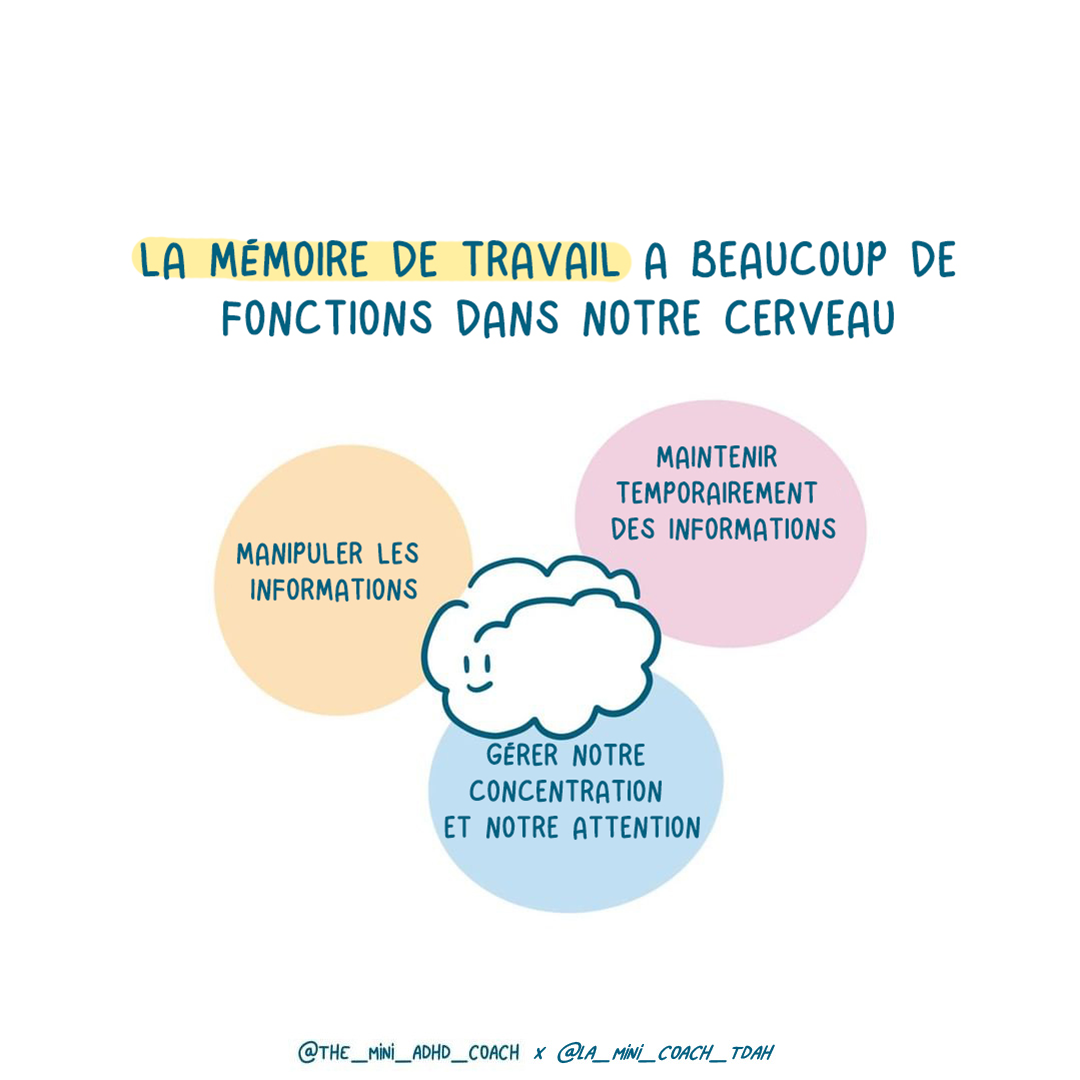
\includegraphics[width=0.7\textwidth]{images/ADHD-Working-Memory.png}
    \caption{Mémoire de Travail (TDAH)}
    \label{fig:tdah}
\end{figure}

\end{document}
